% !TeX program = xelatex
% !TeX encoding = UTF-8
\documentclass[UTF8,fontset=none,a4paper,11pt]{ctexart}

% ---------- fonts ----------
\usepackage{fontspec}
\setCJKmainfont{Noto Serif CJK SC}[BoldFont={Noto Serif CJK SC Bold}]
\setCJKsansfont{Noto Sans CJK SC}[BoldFont={Noto Sans CJK SC Bold}]
\setCJKmonofont{Noto Sans Mono CJK SC}

% ---------- layout ----------
\usepackage[a4paper,top=2.3cm,bottom=2.3cm,left=2.2cm,right=2.2cm]{geometry}
\usepackage{amsmath,amssymb,bm}
\usepackage{graphicx}
\usepackage{booktabs}
\usepackage{siunitx}
\usepackage{array}
\usepackage{tabularx}
\usepackage{multirow}
\usepackage{makecell}
\usepackage{caption}
\usepackage{subcaption}
\usepackage{float}
\usepackage{xcolor}
\usepackage{enumitem}
\usepackage{fancyhdr}
\usepackage[hidelinks]{hyperref}

\sisetup{
  detect-all,
  table-number-alignment=center,
  group-separator={\,},
  group-minimum-digits=4,
  exponent-product=\times,
  output-exponent-marker=\mathrm{e},
  retain-explicit-plus=true,
}
\captionsetup{font=small,labelfont=bf,labelsep=quad}
\setlength{\parindent}{2em}
\setlength{\parskip}{0.25em}
\linespread{1.18}
\setlength{\headheight}{13pt}
\pagestyle{fancy}
\fancyhf{}
\fancyhead[L]{\small\sffamily 楔形变截面矩形拉杆：三种有限元方法与开源锚点}
\fancyhead[R]{\small\thepage}
\renewcommand{\headrulewidth}{0.4pt}
\ctexset{
  section/format = \Large\bfseries\sffamily,
  subsection/format = \large\bfseries\sffamily,
  subsubsection/format = \normalsize\bfseries\sffamily,
}

% ---------- symbols ----------
\newcommand{\dd}{\mathrm{d}}
\newcommand{\ee}{\mathrm{e}}
\newcommand{\bB}{\mathbf{B}}
\newcommand{\bD}{\mathbf{D}}
\newcommand{\bJ}{\mathbf{J}}
\newcommand{\bK}{\mathbf{K}}
\newcommand{\bF}{\mathbf{F}}
\newcommand{\bU}{\mathbf{U}}
\newcommand{\bke}{\mathbf{k}_e}
\newcommand{\beps}{\boldsymbol{\varepsilon}}
\newcommand{\bsig}{\boldsymbol{\sigma}}
\newcommand{\bu}{\mathbf{u}}

\title{\bfseries 楔形变截面矩形拉杆的三种有限元方法与开源锚点对比}
\author{一维变截面杆单元 \quad/\quad Q4 平面应力等参元 \quad/\quad CST 常应变三角形}
\date{2026 年 10 月}

\begin{document}

\maketitle
\thispagestyle{empty}

\begin{abstract}
\noindent
楔形变截面矩形拉杆的轴向刚度与应力分布，是检验一维杆理论适用边界、以及二维单元离散质量的典型问题。本文以截面高度线性变化、关于杆轴对称的矩形拉杆为对象，取 $\beta=0$ 的等截面情形作为退化校核、$\beta=+1.0$ 为主构型，分别实现一维变截面杆单元、四节点双线性等参元 Q4 和三节点常应变三角形 CST，并用 CalculiX 的 CPS4/CPS8 平面应力模型与 FEniCS/dolfinx 作第三方锚点。

数值结果表明：在 $160\times32$ 网格上，Q4 的端部、中截面平均位移相对 CalculiX CPS8（$240\times48$）参考的最大偏差分别为 $0.025\%$ 和 $0.014\%$，探针点应力偏差不超过 $0.042\%$；CST 对应为 $0.075\%$、$0.067\%$ 和 $0.146\%$。Q4 的梯度保真误差为 $0.35\%$–$0.95\%$，位移与应力的观测收敛阶分别约为 $1.7$–$2.5$ 和 $1.6$–$2.3$。CST 的两种对角线剖分在对称工况下互为镜像，端/中位移与截面平均应力是严格不变量（离散度约 $10^{-11}\%$），真正的对角线敏感性只出现在局部单元/节点应力（$160\times32$ 下为 $0.2\%$–$1.1\%$）。

一维杆判据采用 $\eta=|\beta|h_0/L=\tan\alpha$，将工况分为 A（可信）、B（需二维复核）、C（不可信）三级；与 CalculiX 参考相比，一维杆端部偏差依次为 $+0.25\%$、$-0.55\%$、$+0.05\%$、$-3.21\%$、$-7.36\%$，与标签分级一致。CalculiX 同网格 CPS4 与自研 Q4 的端位移差不超过 $0.05\%$；FEniCS 对 S1 的端位移与 CCX 参考仅差 $+0.0029\%$。三种方法在产出形态上的差异——一维曲线、连续云图、分块云图——与它们的精度、自由度和后处理需求同样重要，本文为此单列一节对比。
\end{abstract}

\noindent\textbf{关键词：}变截面杆；平面应力；Q4 等参元；CST；等效刚度；收敛性；CalculiX；对角线敏感性


\newpage
\tableofcontents
\newpage

\section{问题定义与研究内容}

\subsection{研究对象}

变截面杆的轴向响应可以用一维理论以极低代价估算，但其端部与截面内的二维效应会随锥角增大而迅速增强。本文研究一个截面高度沿杆轴线性变化、关于杆轴对称的矩形拉杆：杆轴取 $x$ 轴，$x\in[0,L]$；矩形截面的面外宽度（厚度）$b$ 恒定，面内高度为
\begin{equation}
  h(x)=h_0\left(1+\beta\frac{x}{L}\right),\qquad
  \beta=\frac{h_1-h_0}{h_0},
  \label{eq:taper}
\end{equation}
截面范围为 $y\in[-h(x)/2,\,h(x)/2]$。采用关于杆轴对称、而非“平底楔形”的几何，是为了让截面形心线保持为直线 $y=0$，端部均布轴力的合力通过形心线，不引入额外整体弯曲；$\beta=0$ 即退化为等截面矩形杆。几何与材料参数见表~\ref{tab:params}。

\begin{table}[htbp]
  \centering
  \caption{几何与材料参数。所有量取国际单位制。}
  \label{tab:params}
  \small
  \setlength{\tabcolsep}{3pt}
  \begin{tabular}{@{}llll@{}}
\toprule
参数 & 符号 & {取值} & 单位 \\
\midrule
杆长 & $L$ & 1.0 & m \\
固定端高度 & $h_0$ & 0.2 & m \\
面外厚度 & $b$ & 0.1 & m \\
弹性模量 & $E$ & $2.0\times10^{11}$ & Pa \\
泊松比 & $\nu$ & 0.3 & -- \\
端部总拉力 & $P$ & 1000 & N \\
平面应力厚度 & $t=b$ & 0.1 & m \\
\bottomrule
\end{tabular}

\end{table}

\begin{figure}[htbp]
  \centering
  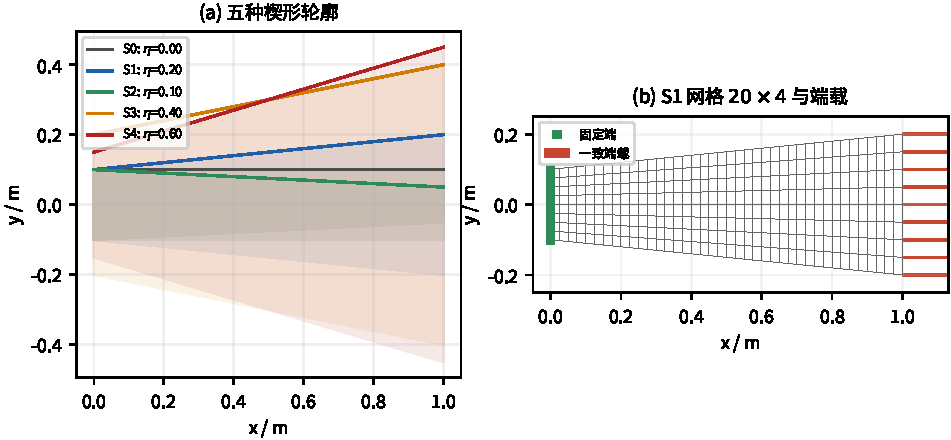
\includegraphics[width=\textwidth]{figures/fig01_geometry_mesh.pdf}
  \caption{五种工况的对称楔形轮廓与 S1 的计算网格。现象：轮廓关于 $y=0$ 对称，网格随 $h(x)$ 缩放，斜边保持直线。解读：对称几何使端部载荷合力通过形心线，避免附加弯曲；沿锥度缩放的网格使单元保持近似正交，便于把锥度效应与网格畸变效应分开。}
  \label{fig:geometry}
\end{figure}

\subsection{计算工况}

主构型 S1 取 $\beta=+1.0$，高度由 $0.2\,\mathrm{m}$ 增至 $0.4\,\mathrm{m}$；S0 为 $\beta=0$ 的退化校核；S2 为收缩楔形，S3、S4 为粗短/极端楔形，用于把一维判据推到 A/B/C 边界。五种工况见表~\ref{tab:cases}。

\begin{table}[htbp]
  \centering
  \caption{五种计算工况。$\eta=|\beta|h_0/L$ 为锥角正切，$A_1/A_0$ 为端部与固定端面积比。}
  \label{tab:cases}
  \small
  \begin{tabular}{@{}lS[table-format=+1.2]S[table-format=1.2]S[table-format=1.2]S[table-format=1.2]S[table-format=2.1]S[table-format=1.2]@{}}
\toprule
工况 & {$\beta$} & {$h_0$/m} & {$h_1$/m} & {$\eta=|\beta|h_0/L$} & {锥角/$^\circ$} & {$A_1/A_0$} \\
\midrule
S0 & +0.00 & 0.20 & 0.20 & 0.00 & 0.0 & 1.00 \\
S1 & +1.00 & 0.20 & 0.40 & 0.20 & 11.3 & 2.00 \\
S2 & -0.50 & 0.20 & 0.10 & 0.10 & 5.7 & 0.50 \\
S3 & +1.00 & 0.40 & 0.80 & 0.40 & 21.8 & 2.00 \\
S4 & +2.00 & 0.30 & 0.90 & 0.60 & 31.0 & 3.00 \\
\bottomrule
\end{tabular}

\end{table}

\subsection{边界条件与载荷}

固定端 $x=0$ 全部节点满足 $u_x=u_y=0$；加载端 $x=L$ 施加沿 $x$ 方向的均布轴向拉力，合力 $P=1000\,\mathrm{N}$；上下斜边自由。二维模型采用平面应力，厚度 $t=b=0.1\,\mathrm{m}$。

端部载荷采用\textbf{均布轴向拉力的一致节点载荷}，而非“每个端节点等分 $P$”的集中载荷：线性边每个微段的面力合力一半分给两端节点，角点因此为内点的一半；CPS8 则按 $1/6$–$2/3$–$1/6$ 分配。两种口径对 $u_{\rm end}$ 的影响不超过 $0.28\%$，但对加载端局部节点应力可达 $1\%$–$8\%$，因此点值应力对比时必须统一。本文所有结果均采用一致面力口径，敏感性在 \S\ref{sec:anchor} 中量化。

\subsection{研究内容}

等参元与常应变三角形的标准推导可参考经典教材~\cite{zienkiewicz2005,bathe2006,hughes2000}。本文完成四项工作。第一，自写 Python+NumPy/SciPy 有限元程序，实现一维变截面杆、Q4 与 CST 的单元刚度、稀疏组装与求解。第二，比较端部/中截面位移、名义应力沿轴曲线与应力误差随网格的 $e$--$\sigma$ 收敛。第三，量化 Q4 的梯度保真误差与剪切能比，以及 CST 的面积加权节点应力恢复与对角线离散度。第四，用 CalculiX CPS4/CPS8 建立第三方锚点，并用 FEniCS 做可选本构校核。三种方法的\textbf{产出形态}差异单列于第~\ref{sec:forms} 节，因为“能输出什么”与“算得多准”同样决定工程选型。
\section{理论与方法}

\subsection{一维变截面杆单元}

轴力沿杆轴守恒，$N(x)=P$，于是名义应力、应变和位移为
\begin{gather}
  \sigma(x)=\frac{P}{A(x)},\qquad
  \varepsilon(x)=\frac{P}{E A(x)},\qquad
  A(x)=b\,h(x), \label{eq:1d-fields}\\
  u(x)=\int_0^x \frac{P}{E A(s)}\,\dd s
      =\frac{P L}{E b h_0\beta}\ln\!\left(1+\beta\frac{x}{L}\right)
      \quad(\beta\neq0), \label{eq:1d-u}
\end{gather}
$\beta=0$ 时式~\eqref{eq:1d-u} 的极限为 $u=Px/(E b h_0)$。

两节点杆单元只有轴向自由度。若单元内轴力为常数 $N_e$，端部相对位移由柔度积分给出
\begin{equation}
  \Delta u_e=N_e\int_{x_1}^{x_2}\frac{\dd x}{E A(x)},
  \qquad
  k_e=\left[\int_{x_1}^{x_2}\frac{\dd x}{E A(x)}\right]^{-1}
      =\frac{E A_0\beta}{L\ln\!\big[(1+\beta x_2/L)/(1+\beta x_1/L)\big]},
  \label{eq:bar-k}
\end{equation}
$\beta\to0$ 时 $k_e\to EA_0/(x_2-x_1)$。对线性 $A(x)$，式~\eqref{eq:bar-k} 等价于面积的对数平均 $A_{\log}=(A_2-A_1)/\ln(A_2/A_1)$；常见的“平均面积刚度”则使用算术平均 $A_{\rm mean}=(A_1+A_2)/2$。由于 $A_{\rm mean}\ge A_{\log}$，平均面积法会高估刚度：$\beta=1$、整杆一个单元时 $k_{\rm mean}/k_e\approx1.0397$，端位移低估约 $3.8\%$。

采用精确柔度积分后，各单元承受同一轴力 $P$，沿杆串联得到
\begin{equation}
  u(x_i)=\sum_{e\le i}\frac{P}{k_e}=\int_0^{x_i}\frac{P}{E A(s)}\,\dd s,
  \label{eq:bar-exact}
\end{equation}
即节点位移与网格无关、与解析解一致。这个性质把“等效刚度是否正确”与“网格是否足够密”分离开，是杆单元在本问题中的核心优势。

\textbf{一维适用性判据。}楔形的几何小参数是锥角正切
\begin{equation}
  \eta=\left|\frac{\dd h}{\dd x}\right|=\frac{|\beta|h_0}{L}=\tan\alpha .
  \label{eq:eta}
\end{equation}
本文取 A 级 $\eta\le0.20$（$\alpha\le11.3^\circ$）、B 级 $0.20<\eta\le0.40$、C 级 $\eta>0.40$。阈值由二维数值解的后验误差标定：A 级内部/中截面偏差一般小于 $0.5\%$、端部边界层约 $1\%$；B 级内部约 $1\%$、端部可达 $4\%$；C 级内部数个百分点、端部接近 $10\%$。

\subsection{Q4 双线性等参元}

四节点四边形在自然坐标 $(\xi,\eta)\in[-1,1]^2$ 内采用双线性形函数
\begin{equation}
  N_i(\xi,\eta)=\frac14(1+\xi_i\xi)(1+\eta_i\eta),\qquad
  (\xi_i,\eta_i)\in\{(-1,-1),(1,-1),(1,1),(-1,1)\}.
\end{equation}
等参映射为 $\mathbf{x}=\sum_iN_i\mathbf{x}_i$，雅可比矩阵 $\bJ$、应变矩阵 $\bB$（$3\times8$）与平面应力本构矩阵 $\bD$ 均为标准形式：
\begin{equation}
  \bB_i=\begin{bmatrix}
    \partial N_i/\partial x & 0\\
    0 & \partial N_i/\partial y\\
    \partial N_i/\partial y & \partial N_i/\partial x
  \end{bmatrix},\qquad
  \bD=\frac{E}{1-\nu^2}
  \begin{bmatrix}
    1 & \nu & 0\\
    \nu & 1 & 0\\
    0 & 0 & (1-\nu)/2
  \end{bmatrix}.
\end{equation}
单元刚度采用 $2\times2$ 高斯全积分：
\begin{equation}
  \bke=\int_{-1}^{1}\int_{-1}^{1}\bB^{\mathrm T}\bD\bB\,t\,|\bJ|\,\dd\xi\,\dd\eta
      \approx\sum_{q=1}^{4}\bB_q^{\mathrm T}\bD\bB_q\,t\,|\bJ_q|.
  \label{eq:q4-ke}
\end{equation}
本文不引入减缩积分。后处理在每个高斯点计算 $\bsig_q=\bD\bB_q\bu_e$，再按 $x$ 列取截面平均。

为评价单元对\textbf{应力梯度}的复现能力，定义梯度保真误差
\begin{equation}
  e_{\rm grad}=
  \frac{\left\|\dfrac{\dd\bar{\sigma}_x}{\dd x}-\dfrac{\dd\bar{\sigma}_{x,\rm ref}}{\dd x}\right\|}
       {\left\|\dfrac{\dd\bar{\sigma}_{x,\rm ref}}{\dd x}\right\|},
  \label{eq:egrad}
\end{equation}
在 $x=0.1L,\ldots,0.9L$ 上用二阶中心差分计算，参考梯度取 CalculiX CPS8 细网格。分子与分母使用同一差分算子，截断误差主项大部分抵消。另定义剪切能比
\begin{equation}
  R_s=\frac{\int(\sigma_y^2+\tau_{xy}^2)\,\dd V}{\int\sigma_x^2\,\dd V},
  \label{eq:Rs}
\end{equation}
作为截面应力偏离单轴应力状态的能量度量，用于辅助一维判据。

\subsection{CST 常应变三角形}

三节点线性位移插值给出常数应变矩阵 $\bB$（$3\times6$）与显式刚度
\begin{equation}
  \bke=t\,|A|\,\bB^{\mathrm T}\bD\bB,\qquad
  \bsig_e=\bD\bB\bu_e,
  \label{eq:cst}
\end{equation}
其中 $|A|$ 为三角形面积。CST 满足完备性与分片试验，但常应变假设使其偏刚，且应力场分段常数、跨单元不连续。

\textbf{面积加权节点恢复。}对共享节点的所有单元作面积加权平均
\begin{equation}
  \bsig_{\rm node}
  =\frac{\sum_{e\ni n}A_e\,\bsig_e}{\sum_{e\ni n}A_e},
  \label{eq:recovery}
\end{equation}
在常应力场中该式精确成立。恢复后的节点应力用于沿轴剖面、截面内离散度与对角线对比，并与未加权算术恢复对照。

\textbf{对角线敏感性与镜像不变量。}矩形网格每个四边形可沿两条对角线之一剖分。本文几何、材料、约束和载荷都关于 $y=0$ 对称，因此两种剖分的解互为镜像：
\begin{equation}
  u_{x,\rm pos}(x,y)=u_{x,\rm neg}(x,-y),\qquad
  \sigma_{x,\rm pos}(x,y)=\sigma_{x,\rm neg}(x,-y),\qquad
  \tau_{xy,\rm pos}(x,y)=-\tau_{xy,\rm neg}(x,-y).
  \label{eq:mirror}
\end{equation}
于是 $u_{\rm end}$、$u_{\rm mid}$、截面平均应力、总能量和反力在两种剖分下严格相等（数值上到舍入误差）。这不是“对角线不敏感”，而是对称性带来的不变量；真正的敏感性在局部场。本文用
\begin{align}
  D_{\sigma,\rm el}&=\frac{\sqrt{\frac1{N_e}\sum_e(\sigma_{x,e,\rm pos}-\sigma_{x,e,\rm neg})^2}}
                          {\sqrt{\frac1{N_e}\sum_e\sigma_{x,e,\rm nom}^2}},\label{eq:Delem}\\
  D_{\sigma,\rm node}&=\frac{\sqrt{\frac1{N_n}\sum_n(\sigma_{x,n,\rm pos}-\sigma_{x,n,\rm neg})^2}}
                            {\frac1{N_n}\sum_n\sigma_{x,n,\rm pos}}\label{eq:Dnode}
\end{align}
量化局部敏感性，并统计截面内节点应力的离散系数 $CV=\mathrm{std}/\mathrm{mean}$，比较 raw 单元常应力、面积加权恢复与算术恢复。

\subsection{第三方锚点与误差口径}

CalculiX~\cite{dhondt2023} 模型直接复用共享网格的节点与四边形：CPS4/CPS8 平面应力单元；厚度由 \texttt{*SOLID} \texttt{SECTION} 第二行给定为 $0.1\,\mathrm{m}$，\texttt{*ELASTIC} 取 $E=2.0\times10^{11}\,\mathrm{Pa}$、$\nu=0.3$；左端全约束，右端施加与自研程序一致的一致面力节点载荷。CPS8 的 $240\times48$ 网格作为二维参考，并用 $80\times16$、$160\times32$ 做参考收敛检查；CPS4 在 $20\times4$ 至 $160\times32$ 上与自研 Q4 做同网格锚点对比。FEniCS/dolfinx 0.11~\cite{alnaes2015,fenicsx} 以 P2 三角形做可选本构校核。

端/中截面位移采用\textbf{面积加权（梯形权重）}平均
\begin{equation}
  \bar u(x)=\frac1{h(x)}\int_{-h(x)/2}^{h(x)/2}u_x(x,y)\,\dd y,
  \label{eq:ubar}
\end{equation}
不使用节点算术平均，因为含边中点时端点权重不对，会引入 $O(1/n_y)$ 的虚假偏差。相对误差统一为 $e=|a-b|/|b|$。收敛阶由 $\log e$--$\log h$ 在 $40\times8$、$80\times16$、$160\times32$ 三个网格上线性拟合。应力误差分两类：截面平均应力误差主要检验平衡与积分一致性，探针点应力误差则检验二维应力分布。探针点取 $x/L=0.1,0.2,0.5,0.8,0.9$ 与 $y/h=0,\pm1/4$，参考值取 CPS8 $240\times48$ 的对应节点。
\section{三种方法的产出形态对比}
\label{sec:forms}

三种方法最本质的差别并不只在数值精度，而在\textbf{产出形态}：一维杆只给出一条轴向曲线，Q4 给出连续二维场，CST 给出分块常应力场。表~\ref{tab:forms} 从未知量、应力表示、主要产出和后处理能力四个维度归纳这一差异；图~\ref{fig:forms} 用同一 S1 工况、同一 $40\times8$ 网格并排展示三种产出。

\begin{table}[htbp]
  \centering
  \caption{三种方法的产出形态对比。表中的“信息量”指对截面内应力分布与端部局部变形的描述能力，而非数值精度。}
  \label{tab:forms}
  \footnotesize
  \begin{tabular}{@{}p{0.17\textwidth}p{0.25\textwidth}p{0.25\textwidth}p{0.25\textwidth}@{}}
\toprule
维度 & 一维杆单元 & Q4 等参元 & CST 三角形 \\
\midrule
每节点自由度 & 1（$u_x$） & 2（$u_x,u_y$） & 2（$u_x,u_y$） \\
单元未知量 & 2 & 8 & 6 \\
单元刚度 & $2\times2$，闭式 & $8\times8$，$2\times2$ 高斯积分 & $6\times6$，显式 \\
应力表示 & 单元常数（按平衡恢复） & 单元内双线性 & 单元常数（常应变） \\
主要产出 & $u(x)$、$\sigma(x)$ 两条一维曲线 & 连续 $\sigma_x$ 云图、任意点应力 & 分块 $\sigma_x$ 云图、节点恢复场 \\
信息量/代价 & 信息最少、自由度最省 & 场连续、代价中等 & 单元数约为 Q4 两倍，局部应力不连续 \\
后处理 & 截面平均、1D 判据 & 高斯点应力、梯度保真、剪切能比 & 面积加权恢复、对角线离散 \\
典型适用 & 杆系快速估算、A/B 级工况 & 光滑二维场、端部复核 & 复杂几何、快速原型 \\
\bottomrule
\end{tabular}

\end{table}

\begin{figure}[htbp]
  \centering
  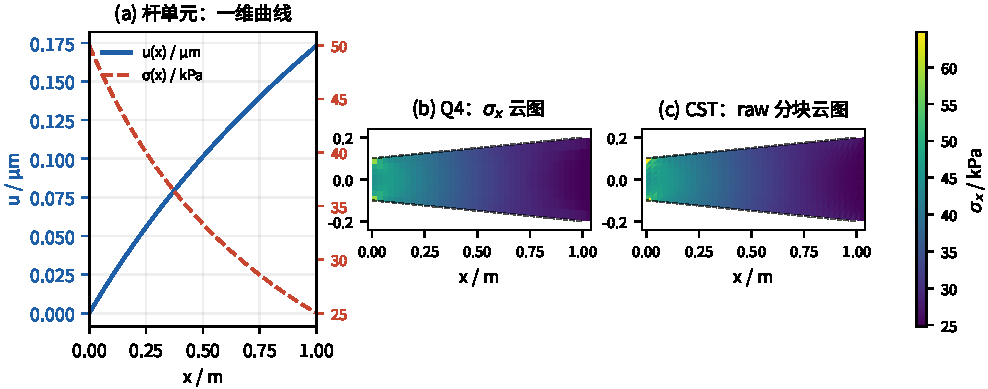
\includegraphics[width=\textwidth]{figures/fig_production_forms.pdf}
  \caption{同一 S1 工况（$40\times8$）下三种方法的产出形态。现象：杆单元只产生 $u(x)$、$\sigma(x)$ 两条一维曲线；Q4 云图在单元内与跨单元均连续；CST raw 云图呈明显分块，块界即单元边界。解读：曲线形式自由度最省、信息量最低，适合一维杆系快速估算；Q4 的双线性插值与高斯点应力给出连续场，适合光滑应力场与端部复核；CST 的常应变假设导致分块，需面积加权节点恢复或更密网格才能得到平滑场，这也是后文单独量化对角线离散度的原因。}
  \label{fig:forms}
\end{figure}

产出形态差异带来三点直接后果。第一，评价指标必须与产出形态匹配：杆单元应比较截面平均位移/应力与一维判据，Q4/CST 则应比较二维点值或全场误差；若只用端部位移，会掩盖 CST 局部应力的分块误差。第二，CST 的“raw 云图”不能直接作为应力结果使用，面积加权节点恢复或更密网格是必要的后处理；本文因此同时报告 raw 与 recovered 两套剖面。第三，若工程只关心轴力与截面平均应力，一维杆的曲线已足够；若关心端部应力集中、楔形边缘的横向应力或局部屈服，则必须使用 Q4 或更密 CST。图~\ref{fig:forms}(b) 与 (c) 的视觉差异，正是第~\ref{sec:results} 节精度差异的直观来源。

\section{程序实现与验证}

\subsection{程序结构}

程序用 Python+NumPy/SciPy 从零实现，不调用现成有限元库。共享核心负责几何、网格、稀疏组装与边界处理，三种方法各自维护单元刚度与后处理：\texttt{fem/config.py} 定义几何、材料、工况与站位；\texttt{fem/analytic.py} 给出一维解析解与闭式等效刚度；\texttt{fem/mesh.py} 生成关于杆轴对称的结构化楔形网格及 Q4/CST 两种剖分；\texttt{fem/assembly.py} 完成稀疏组装、Dirichlet 消元与一致端载；\texttt{fem/post.py} 实现面积加权的截面平均位移；\texttt{fem/bar.py}、\texttt{fem/q4.py}、\texttt{fem/cst.py} 分别实现三种方法；\texttt{anchors/calculix} 负责 CalculiX 输入生成、运行与 \texttt{.dat/.frd} 解析，\texttt{anchors/fenics} 为可选本构校核。所有结果由 \texttt{scripts/} 下的驱动脚本一键复现。

\subsection{验证}

下列校核全部通过（67 项自动测试）：解析极限（$\beta=0$ 时一维解等于 $PL/(EA)$、等效刚度退化为 $EA/L$、柔度串联可加）；Q4/CST 常应变分片试验（线性位移场下应力等于 $\bD\beps$）；刚体平移零应力；反力校核（固定端反力等于 $-P$，Q4/CST 最大相对误差约 $10^{-12}$）；杆单元节点精确性（与解析解差约 $10^{-13}$）；CST 镜像不变量（两种对角线剖分的 $u_{\rm end}$、$u_{\rm mid}$、截面平均应力差约 $10^{-11}\%$）。这些校核保证后续差异来自离散方法本身，而非实现错误。

\subsection{与 CalculiX 的同网格交叉校核}

同网格 CPS4 与自研 Q4 的端位移相对差最大 $0.049\%$（均值 $0.017\%$），截面平均应力差小于 $0.006\%$；同网格 CST 与 CPS4 的端位移差在粗网格最大 $0.46\%$，到 $160\times32$ 降到 $0.001\%$ 量级。差异来自 CalculiX 平面应力单元的内部三维展开与厚度积分细节，属于锚点可接受范围。FEniCS 的 P2 三角形结果进一步独立验证了 S0/S1 的位移与应力量级（见 \S\ref{sec:fenics}）。

\section{结果与对比}
\label{sec:results}

\subsection{端部与中截面位移}

Q4 与 CST 在 $160\times32$ 网格上均已高度接近 CalculiX 参考；一维杆只在 A 级工况可信。五种工况的端/中截面平均位移见 表~\ref{tab:disp-end} 与 表~\ref{tab:disp-mid}，相对 CCX 参考的偏差见 表~\ref{tab:dev}。Q4 的端/中位移最大偏差为 $0.025\%/0.014\%$，CST 为 $0.075\%/0.067\%$。相对一维解，S0、S1、S2 的偏差在 $0.6\%$ 以内；S3 端部偏差约 $3.3\%$，S4 约 $7.9\%$，已超出工程可接受范围。

\begin{table}[htbp]
  \centering
  \caption{端截面平均位移 $u_{\rm end}$（$\si{\micro\metre}$，$160\times32$ 网格）。}
  \label{tab:disp-end}
  \small
  \begin{tabular}{@{}lS[table-format=1.6]S[table-format=1.6]S[table-format=1.6]S[table-format=1.6]S[table-format=1.6]@{}}
\toprule
工况 & {1D} & {杆} & {Q4} & {CST} & {CCX CPS8} \\
\midrule
S0 & 0.250000 & 0.250000 & 0.249379 & 0.249368 & 0.249380 \\
S1 & 0.173287 & 0.173287 & 0.174238 & 0.174220 & 0.174238 \\
S2 & 0.346574 & 0.346574 & 0.346400 & 0.346390 & 0.346395 \\
S3 & 0.086643 & 0.086643 & 0.089506 & 0.089480 & 0.089520 \\
S4 & 0.091551 & 0.091551 & 0.098794 & 0.098745 & 0.098819 \\
\bottomrule
\end{tabular}

\end{table}

\begin{table}[htbp]
  \centering
  \caption{中截面平均位移 $u_{\rm mid}$（$\si{\micro\metre}$，$160\times32$ 网格）。}
  \label{tab:disp-mid}
  \small
  \begin{tabular}{@{}lS[table-format=1.6]S[table-format=1.6]S[table-format=1.6]S[table-format=1.6]S[table-format=1.6]@{}}
\toprule
工况 & {1D} & {杆} & {Q4} & {CST} & {CCX CPS8} \\
\midrule
S0 & 0.125000 & 0.125000 & 0.124379 & 0.124368 & 0.124380 \\
S1 & 0.101366 & 0.101366 & 0.101423 & 0.101406 & 0.101420 \\
S2 & 0.143841 & 0.143841 & 0.143423 & 0.143413 & 0.143429 \\
S3 & 0.050683 & 0.050683 & 0.051273 & 0.051253 & 0.051280 \\
S4 & 0.057762 & 0.057762 & 0.060221 & 0.060189 & 0.060229 \\
\bottomrule
\end{tabular}

\end{table}

\begin{table}[htbp]
  \centering
  \caption{相对 CalculiX CPS8 $240\times48$ 参考的偏差（$160\times32$，单位：\%）。$e_{\rm end}$、$e_{\rm mid}$ 为位移偏差，$e_\sigma$ 为探针点应力偏差。一维杆的偏差定义为 $(u_{\rm bar}-u_{\rm ref})/u_{\rm ref}$。}
  \label{tab:dev}
  \footnotesize
  \setlength{\tabcolsep}{4pt}
  \begin{tabular}{@{}lS[table-format=+1.2]S[table-format=+1.4]S[table-format=+1.4]S[table-format=+1.4]S[table-format=+1.4]S[table-format=1.4]S[table-format=1.4]@{}}
\toprule
工况 & {杆 $e_{\rm end}$} & {Q4 $e_{\rm end}$} & {Q4 $e_{\rm mid}$} & {CST $e_{\rm end}$} & {CST $e_{\rm mid}$} & {Q4 $e_\sigma$} & {CST $e_\sigma$} \\
\midrule
S0 & +0.249 & -0.0002 & -0.0004 & -0.0047 & -0.0095 & 0.0183 & 0.0258 \\
S1 & -0.546 & -0.0002 & +0.0029 & -0.0106 & -0.0137 & 0.0197 & 0.0372 \\
S2 & +0.052 & +0.0016 & -0.0040 & -0.0014 & -0.0105 & 0.0147 & 0.0200 \\
S3 & -3.214 & -0.0156 & -0.0140 & -0.0450 & -0.0535 & 0.0417 & 0.1019 \\
S4 & -7.355 & -0.0251 & -0.0141 & -0.0752 & -0.0667 & 0.0395 & 0.1458 \\
\bottomrule
\end{tabular}

\end{table}

\begin{figure}[htbp]
  \centering
  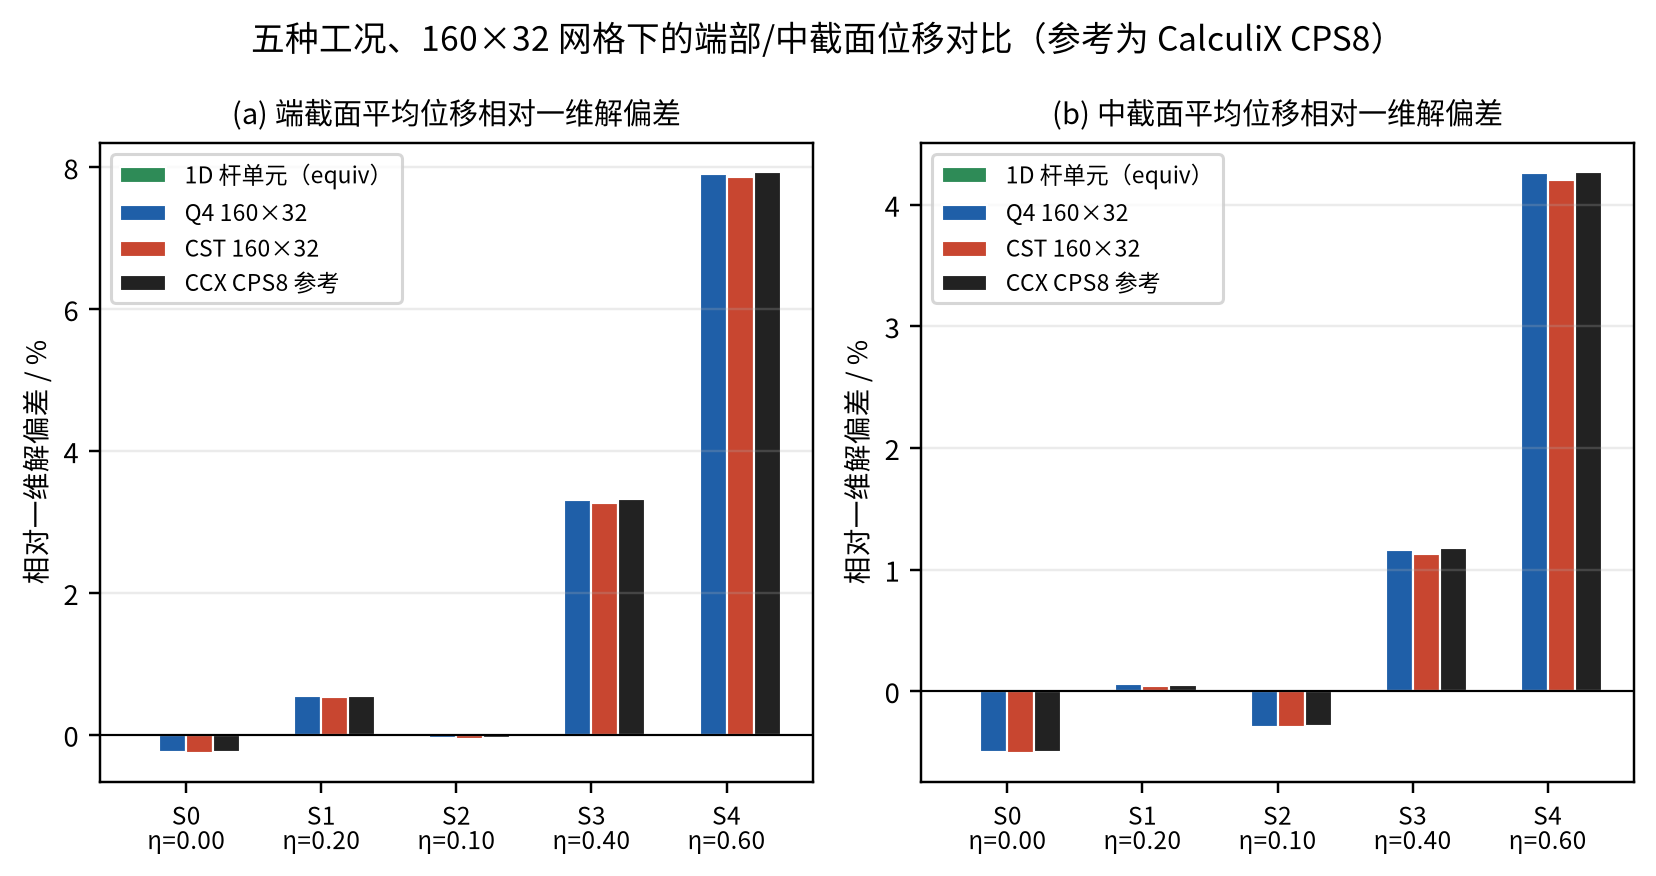
\includegraphics[width=\textwidth]{figures/fig02_displacement.png}
  \caption{五种工况在 $160\times32$ 网格下的端/中截面位移相对一维解的偏差。现象：S0、S1、S2 的偏差在 $1\%$ 以内，S3、S4 的偏差随 $\eta$ 迅速增大；Q4、CST 与 CCX 参考的柱高几乎重合。解读：小锥角下二维效应主要是端部边界层，一维名义解仍可用；大锥角下横向应力与楔形边缘效应成为一阶量，一维杆失效，而 Q4/CST 仍能跟踪参考。}
  \label{fig:displacement}
\end{figure}

值得注意的是，S0（$\beta=0$）的一维解与二维参考也有约 $0.25\%$ 的端部偏差、$0.50\%$ 的中截面偏差。这不是锥度效应，而是固定端全约束阻止泊松收缩造成的真实边界层；即便等截面杆，若关心端部位移，也应使用二维模型或至少做端部修正。

\subsection{名义应力沿轴曲线}

截面平均应力由平衡决定，任何满足平衡的离散解都应逼近 $\sigma_{\rm nom}=P/A(x)$；二维效应体现在应力沿截面的\textbf{非均匀分布}上。表~\ref{tab:stress-profile} 显示，S1 的内部截面平均值与 $P/A(x)$ 的差异在 $0.01\%$ 量级；表~\ref{tab:point-stress} 则显示，$y=0$ 处点应力在固定端附近比名义值高约 $1.8\%$，到中截面仍高约 $0.7\%$。图~\ref{fig:stress} 把这一差异画成沿轴曲线与截面分布。

\begin{table}[htbp]
  \centering
  \caption{S1 的截面平均轴向应力（kPa，$160\times32$）。内部站（$x/L=0.1$–$0.9$）的截面平均与名义值几乎重合。}
  \label{tab:stress-profile}
  \small
  \begin{tabular}{@{}S[table-format=1.1]S[table-format=2.2]S[table-format=2.2]S[table-format=2.2]S[table-format=2.2]@{}}
\toprule
{$x/L$} & {$\sigma_{\rm nom}$/kPa} & {CCX 截面平均/kPa} & {Q4 截面平均/kPa} & {CST 截面平均/kPa} \\
\midrule
0.1 & 45.45 & 45.45 & 45.45 & 45.45 \\
0.2 & 41.67 & 41.67 & 41.67 & 41.67 \\
0.3 & 38.46 & 38.46 & 38.46 & 38.46 \\
0.4 & 35.71 & 35.71 & 35.71 & 35.71 \\
0.5 & 33.33 & 33.33 & 33.33 & 33.33 \\
0.6 & 31.25 & 31.25 & 31.25 & 31.25 \\
0.7 & 29.41 & 29.41 & 29.41 & 29.41 \\
0.8 & 27.78 & 27.78 & 27.78 & 27.78 \\
0.9 & 26.32 & 26.32 & 26.32 & 26.32 \\
\bottomrule
\end{tabular}

\end{table}

\begin{table}[htbp]
  \centering
  \caption{S1 在 $y=0$ 处的轴向应力（kPa，$160\times32$）。参考值为 CalculiX CPS8 $240\times48$。}
  \label{tab:point-stress}
  \small
  \begin{tabular}{@{}S[table-format=1.1]S[table-format=2.2]S[table-format=2.2]S[table-format=2.2]@{}}
\toprule
{$x/L$} & {Q4 $\sigma_x(y=0)$/kPa} & {CST $\sigma_x(y=0)$/kPa} & {CCX $\sigma_x(y=0)$/kPa} \\
\midrule
0.1 & 46.28 & 46.27 & 46.30 \\
0.2 & 42.27 & 42.26 & 42.27 \\
0.5 & 33.55 & 33.55 & 33.55 \\
0.8 & 27.36 & 27.37 & 27.37 \\
0.9 & 25.60 & 25.61 & 25.61 \\
\bottomrule
\end{tabular}

\end{table}

\begin{figure}[htbp]
  \centering
  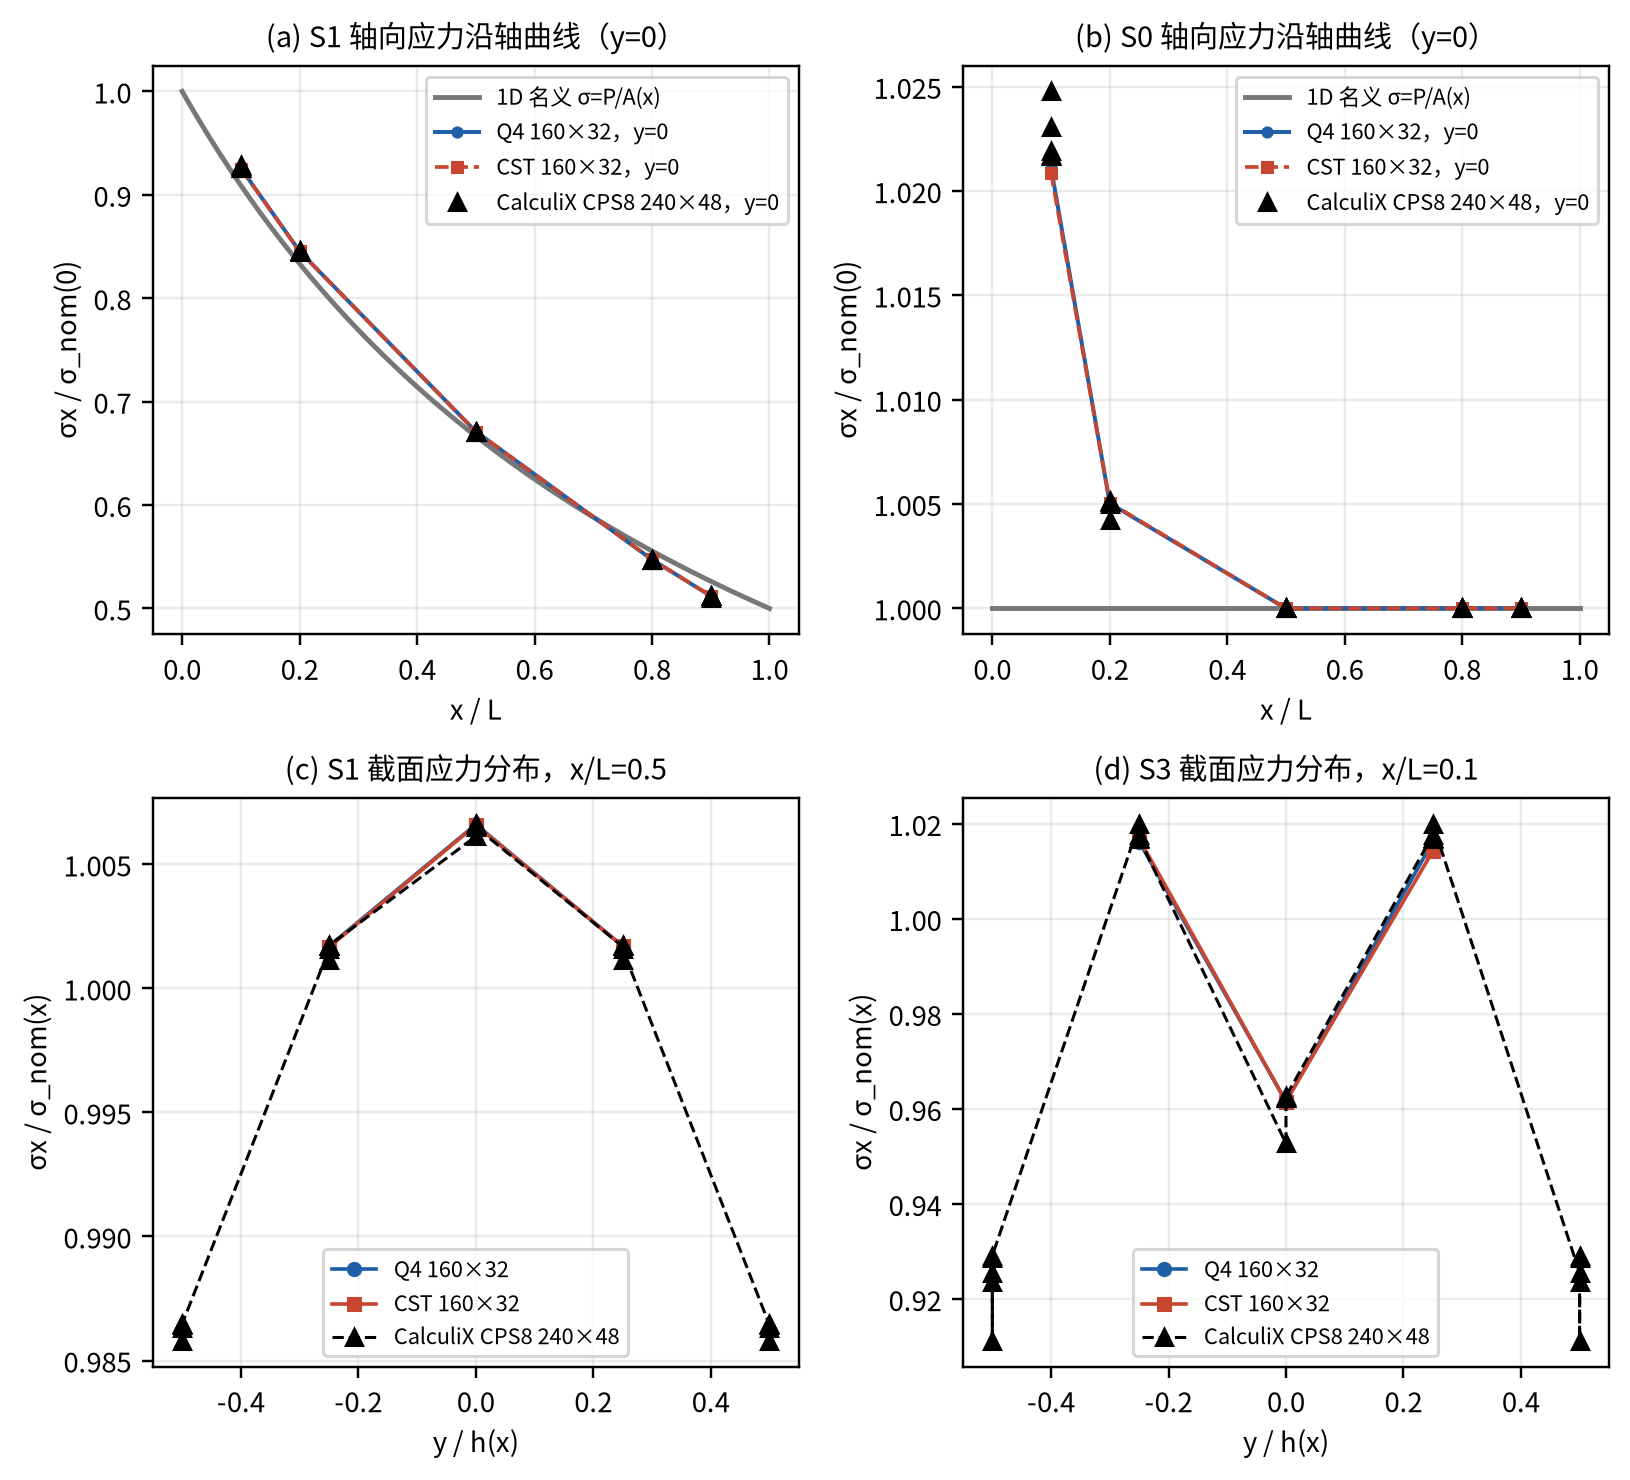
\includegraphics[width=\textwidth]{figures/fig03_stress_profile.png}
  \caption{轴向应力沿轴曲线与截面应力分布。现象：S1 的 $\sigma_x$ 沿轴由约 $50\,\mathrm{kPa}$ 平滑降至 $25\,\mathrm{kPa}$；Q4、CST 与 CCX 在 $y=0$ 处几乎重合，但 CST 在截面边缘略低；S3 的近固定端截面呈明显的“中间低、两侧高”分布。解读：截面平均应力由平衡控制，因而各方法一致；点应力差异反映二维楔形效应与端部约束，S3/S4 的截面非均匀性显著增强，正是一维判据失效的微观表现。}
  \label{fig:stress}
\end{figure}

\subsection{应力与位移收敛}

Q4、CST 的应力和位移误差均随网格单调下降；Q4 的应力阶略高，CST 的局部应力误差更大但同样稳定收敛。应力误差与拟合阶列于 表~\ref{tab:conv}，双对数曲线见图~\ref{fig:conv}。Q4 的探针应力误差为 $0.015\%$–$0.042\%$，CST 为 $0.020\%$–$0.146\%$；Q4 的位移观测阶约 $1.7$–$2.5$（S1 端部因误差已接近参考精度呈超收敛），CST 约 $1.5$–$2.4$。

\begin{table}[htbp]
  \centering
  \caption{应力误差与观测收敛阶。$e$ 为 $160\times32$ 的相对误差（\%），$p$ 由 $40\times8$、$80\times16$、$160\times32$ 三点拟合。CST 的梯度保真误差未定义，以“--”表示。}
  \label{tab:conv}
  \footnotesize
  \setlength{\tabcolsep}{3.5pt}
  \begin{tabular}{@{}llS[table-format=1.4]S[table-format=1.2]S[table-format=1.5]S[table-format=1.2]S[table-format=1.3]S[table-format=1.2]@{}}
\toprule
工况 & 方法 & {$e_{\sigma,\rm probe}$/\%} & {$p_{\rm probe}$} & {$e_{\sigma,\rm profile}$/\%} & {$p_{\rm profile}$} & {$e_{\rm grad}$/\%} & {$p_{\rm grad}$} \\
\midrule
S0 & Q4 & 0.0183 & 1.05 & 0.00007 & 0.00 & \multicolumn{1}{c}{--} & \multicolumn{1}{c}{--} \\
S0 & CST & 0.0258 & 1.32 & 0.00007 & -0.00 & \multicolumn{1}{c}{--} & \multicolumn{1}{c}{--} \\
S1 & Q4 & 0.0197 & 1.58 & 0.00040 & 2.23 & 0.633 & 1.27 \\
S1 & CST & 0.0372 & 1.67 & 0.00039 & 2.27 & \multicolumn{1}{c}{--} & \multicolumn{1}{c}{--} \\
S2 & Q4 & 0.0147 & 0.83 & 0.00025 & 2.55 & 0.347 & 1.65 \\
S2 & CST & 0.0200 & 1.21 & 0.00020 & 2.63 & \multicolumn{1}{c}{--} & \multicolumn{1}{c}{--} \\
S3 & Q4 & 0.0417 & 1.85 & 0.00127 & 1.46 & 0.945 & 1.04 \\
S3 & CST & 0.1019 & 1.60 & 0.00127 & 1.56 & \multicolumn{1}{c}{--} & \multicolumn{1}{c}{--} \\
S4 & Q4 & 0.0395 & 2.04 & 0.00211 & 1.88 & 0.899 & 1.25 \\
S4 & CST & 0.1458 & 1.62 & 0.00203 & 1.97 & \multicolumn{1}{c}{--} & \multicolumn{1}{c}{--} \\
\bottomrule
\end{tabular}

\end{table}

\begin{figure}[htbp]
  \centering
  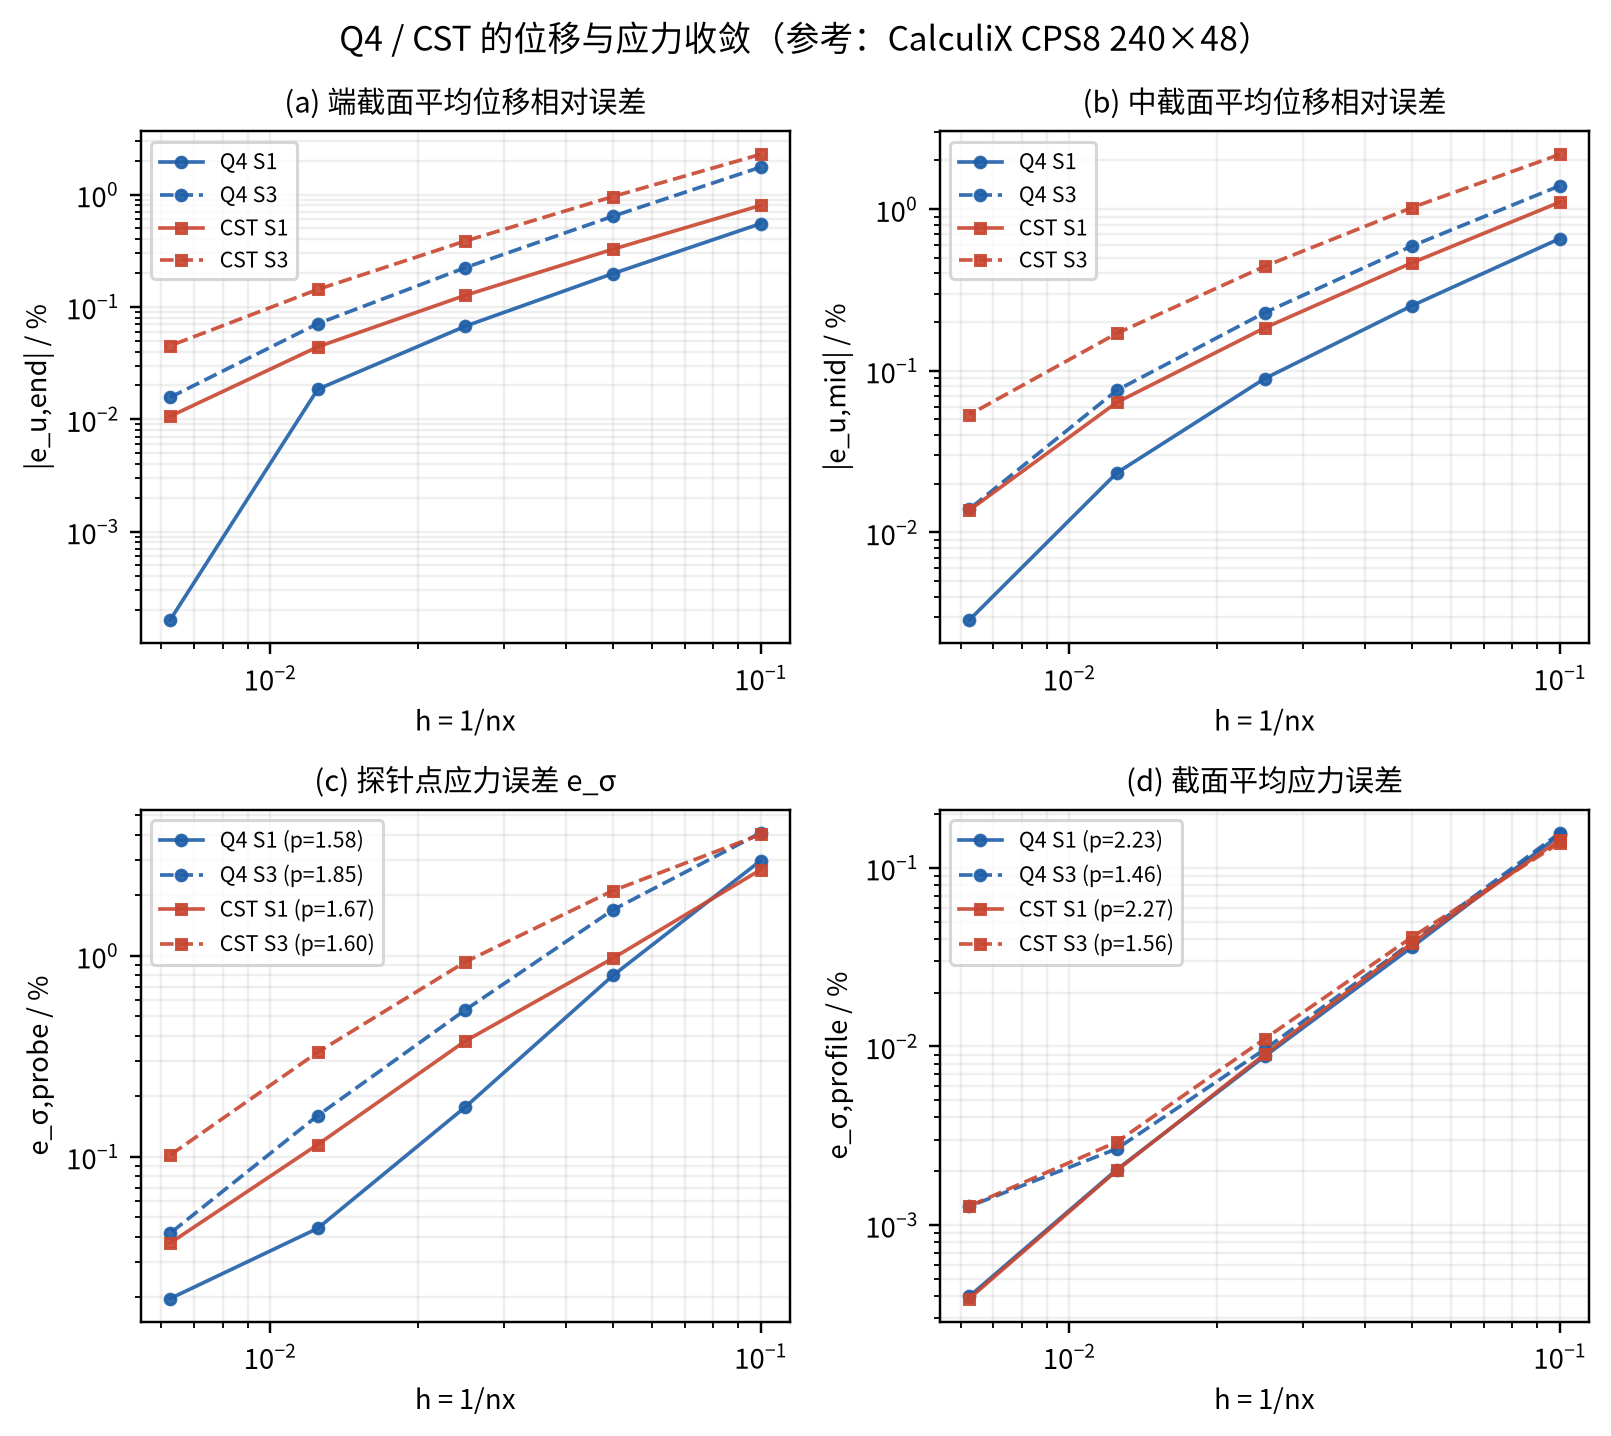
\includegraphics[width=\textwidth]{figures/fig04_convergence.png}
  \caption{Q4/CST 的位移与应力误差随 $h=1/n_x$ 的变化。现象：四个子图的误差均随 $h$ 减小而下降，应力子图的拟合阶集中在 $1.6$–$2.3$；位移子图在细网格端趋于平缓。解读：应力采用点值探针，误差量级更小且阶数稳定；位移误差在细网格受参考解精度与端部边界层限制，拟合阶出现分散，不宜单独作为方法精度判据。}
  \label{fig:conv}
\end{figure}

\subsection{梯度保真与剪切能比}

Q4 对截面平均应力梯度的复现误差为 $0.35\%$–$0.95\%$，随网格以约 $1.0$–$1.7$ 阶下降；剪切能比 $R_s$ 随 $\eta$ 单调增大，定量印证了一维判据。这组结果列于 表~\ref{tab:grad}，并绘于 图~\ref{fig:grad}。

\begin{table}[htbp]
  \centering
  \caption{Q4 的梯度保真误差 $e_{\rm grad}$、拟合阶 $p_{\rm grad}$ 与剪切能比 $R_s$（$160\times32$）。S0 的名义梯度为零，$e_{\rm grad}$ 无定义。}
  \label{tab:grad}
  \small
  \begin{tabular}{@{}lS[table-format=1.2]S[table-format=1.3]S[table-format=1.2]S[table-format=1.3]@{}}
\toprule
工况 & {$\eta$} & {$e_{\rm grad}$/\%} & {$p_{\rm grad}$} & {$R_s$/\%} \\
\midrule
S0 & 0.00 & \multicolumn{1}{c}{--} & \multicolumn{1}{c}{--} & 0.177 \\
S1 & 0.20 & 0.633 & 1.27 & 0.643 \\
S2 & 0.10 & 0.347 & 1.65 & 0.215 \\
S3 & 0.40 & 0.945 & 1.04 & 2.393 \\
S4 & 0.60 & 0.899 & 1.25 & 4.870 \\
\bottomrule
\end{tabular}

\end{table}

\begin{figure}[htbp]
  \centering
  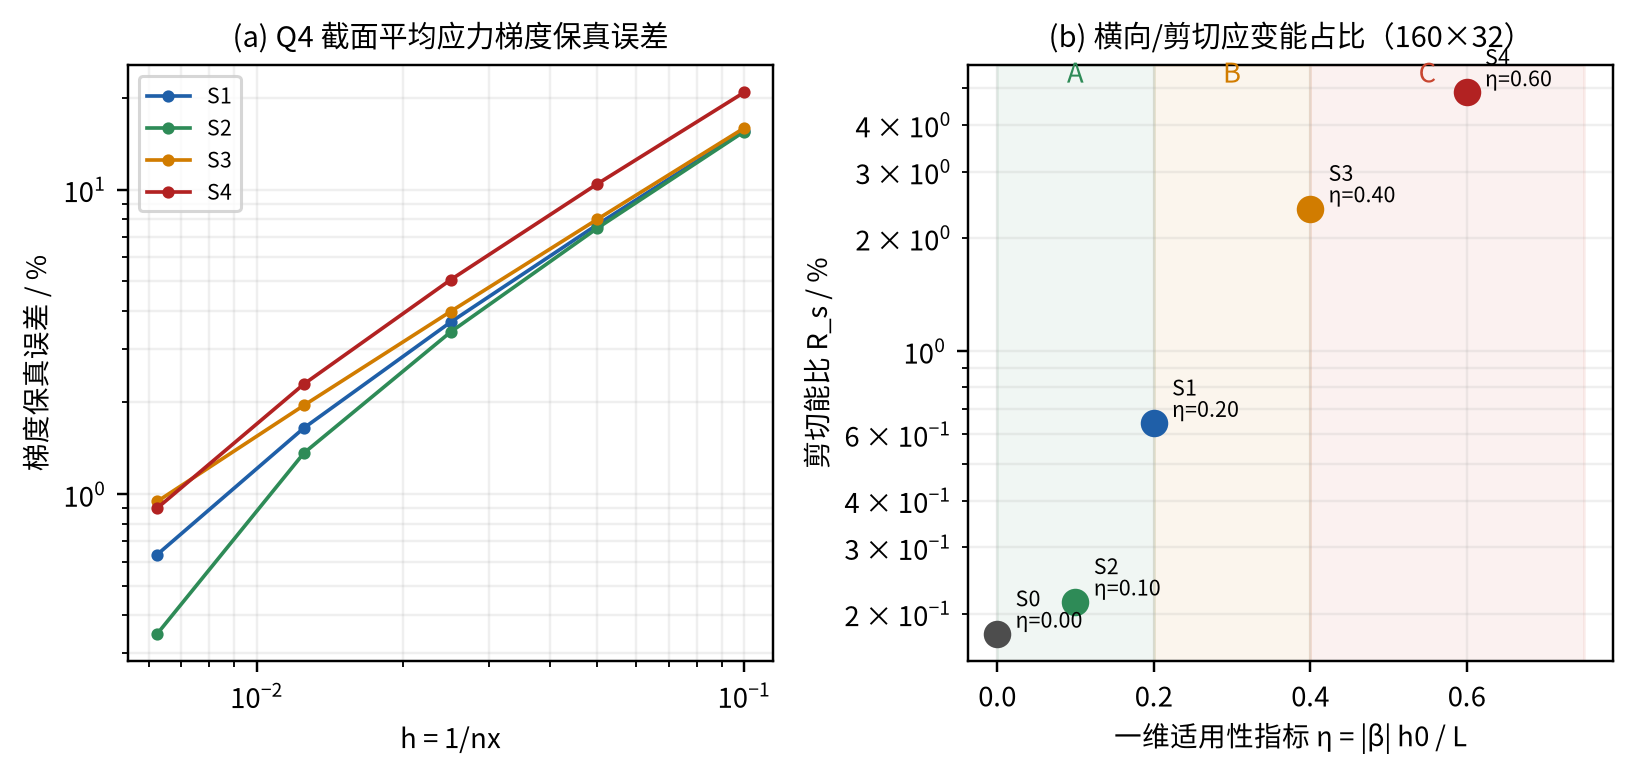
\includegraphics[width=\textwidth]{figures/fig05_gradient_shear.png}
  \caption{梯度保真误差与剪切能比。现象：$e_{\rm grad}$ 随 $h$ 下降，$R_s$ 随 $\eta$ 从 S0 的 $0.18\%$ 增至 S4 的 $4.87\%$。解读：前者说明 Q4 的线性应力场能稳定复现截面平均应力的梯度；后者说明大锥角下横向/剪切能量占比显著上升，一维单轴假设不再成立。}
  \label{fig:grad}
\end{figure}

\subsection{CST 对角线离散度与面积加权恢复}

CST 的全局量对剖分方向不敏感，但局部应力敏感：端/中位移与截面平均应力的对角线离散度为 $10^{-11}\%$ 量级，而单元应力与恢复后节点应力的局部离散度在 $160\times32$ 下为 $0.24\%$–$1.07\%$ 与 $0.31\%$–$2.47\%$。具体对比见表~\ref{tab:diag} 与图~\ref{fig:diag}。

\begin{table}[htbp]
  \centering
  \caption{CST 对角线离散度与截面内离散系数（$160\times32$）。$D_u$、$D_{\sigma,\rm ax}$ 为镜像不变量，理论上应为零；$D_{\sigma,\rm el}$、$D_{\sigma,\rm node}$ 为局部敏感度。}
  \label{tab:diag}
  \footnotesize
  \setlength{\tabcolsep}{3pt}
  \begin{tabular}{@{}lS[table-format=1.2e-2]S[table-format=1.2e-2]S[table-format=1.3]S[table-format=1.3]S[table-format=2.2]S[table-format=2.2]@{}}
\toprule
工况 & {$D_u$/\%} & {$D_{\sigma,\rm ax}$/\%} & {$D_{\sigma,\rm el}$/\%} & {$D_{\sigma,\rm node}$/\%} & {$CV_{\rm raw}$/\%} & {$CV_{\rm rec}$/\%} \\
\midrule
S0 & 6.26e-12 & 1.63e-11 & 0.293 & 0.508 & 2.12 & 2.22 \\
S1 & 1.52e-11 & 1.72e-11 & 0.527 & 1.025 & 3.20 & 3.38 \\
S2 & 2.04e-11 & 2.11e-11 & 0.235 & 0.308 & 2.46 & 2.56 \\
S3 & 7.65e-12 & 1.02e-11 & 0.570 & 1.659 & 6.61 & 7.09 \\
S4 & 6.88e-12 & 8.13e-12 & 1.069 & 2.466 & 9.54 & 10.06 \\
\bottomrule
\end{tabular}

\end{table}

\begin{figure}[htbp]
  \centering
  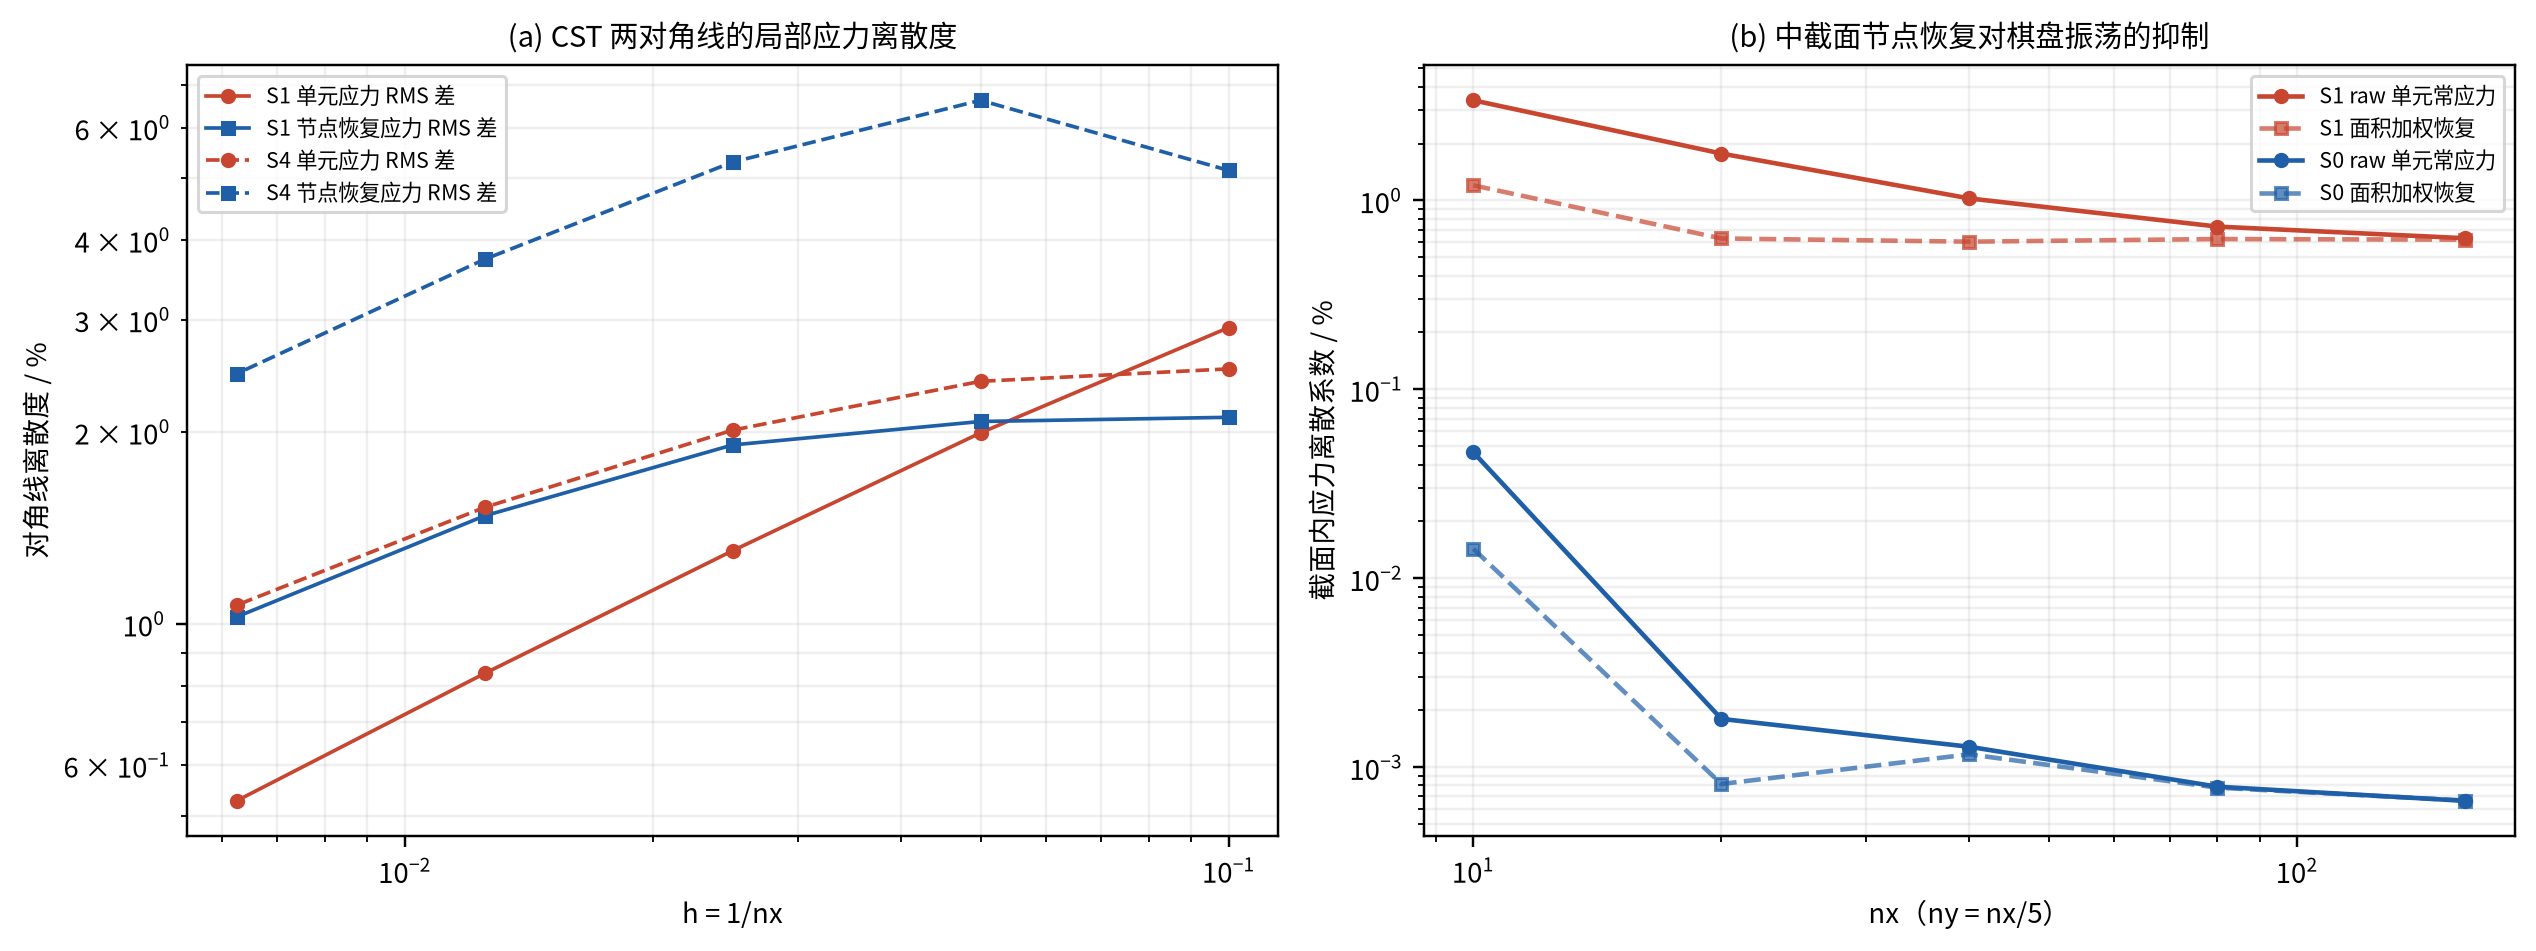
\includegraphics[width=\textwidth]{figures/fig06_cst_diagonal.png}
  \caption{CST 对角线离散度与节点恢复。现象：局部应力离散度随网格下降，S4 的离散度显著高于 S1；面积加权恢复在粗网格上降低了截面内 $CV$，细网格上与 raw 接近。解读：对称工况下剖分方向只影响局部场，不影响全局位移；面积加权恢复主要抑制粗网格的棋盘振荡，不能替代网格加密。}
  \label{fig:diag}
\end{figure}

\subsection{一维杆适用性判据与可信度标签}

一维杆的等效刚度若采用柔度积分，节点位移与解析解一致到 $10^{-13}$ 且与网格无关；用平均面积刚度则会在粗网格下高估刚度、低估端位移。各工况的标签与后验偏差列于 表~\ref{tab:bar}，判据区间见图~\ref{fig:bar}。S0/S1/S2 判为 A，S3 为 B，S4 为 C；端部偏差依次为 $+0.25\%$、$-0.55\%$、$+0.05\%$、$-3.21\%$、$-7.36\%$，与标签分级一致。

\begin{table}[htbp]
  \centering
  \caption{一维杆可信度标签与后验校核。偏差定义为 $(u_{\rm bar}-u_{\rm ccx})/u_{\rm ccx}$（\%）。}
  \label{tab:bar}
  \small
  \begin{tabular}{@{}lS[table-format=1.2]S[table-format=2.1]cS[table-format=+1.2]S[table-format=+1.2]@{}}
\toprule
工况 & {$\eta$} & {锥角/$^\circ$} & 标签 & {端部偏差/\%} & {中截面偏差/\%} \\
\midrule
S0 & 0.00 & 0.0 & A & +0.25 & +0.50 \\
S1 & 0.20 & 11.3 & A & -0.55 & -0.05 \\
S2 & 0.10 & 5.7 & A & +0.05 & +0.29 \\
S3 & 0.40 & 21.8 & B & -3.21 & -1.16 \\
S4 & 0.60 & 31.0 & C & -7.36 & -4.10 \\
\bottomrule
\end{tabular}

\end{table}

\begin{figure}[htbp]
  \centering
  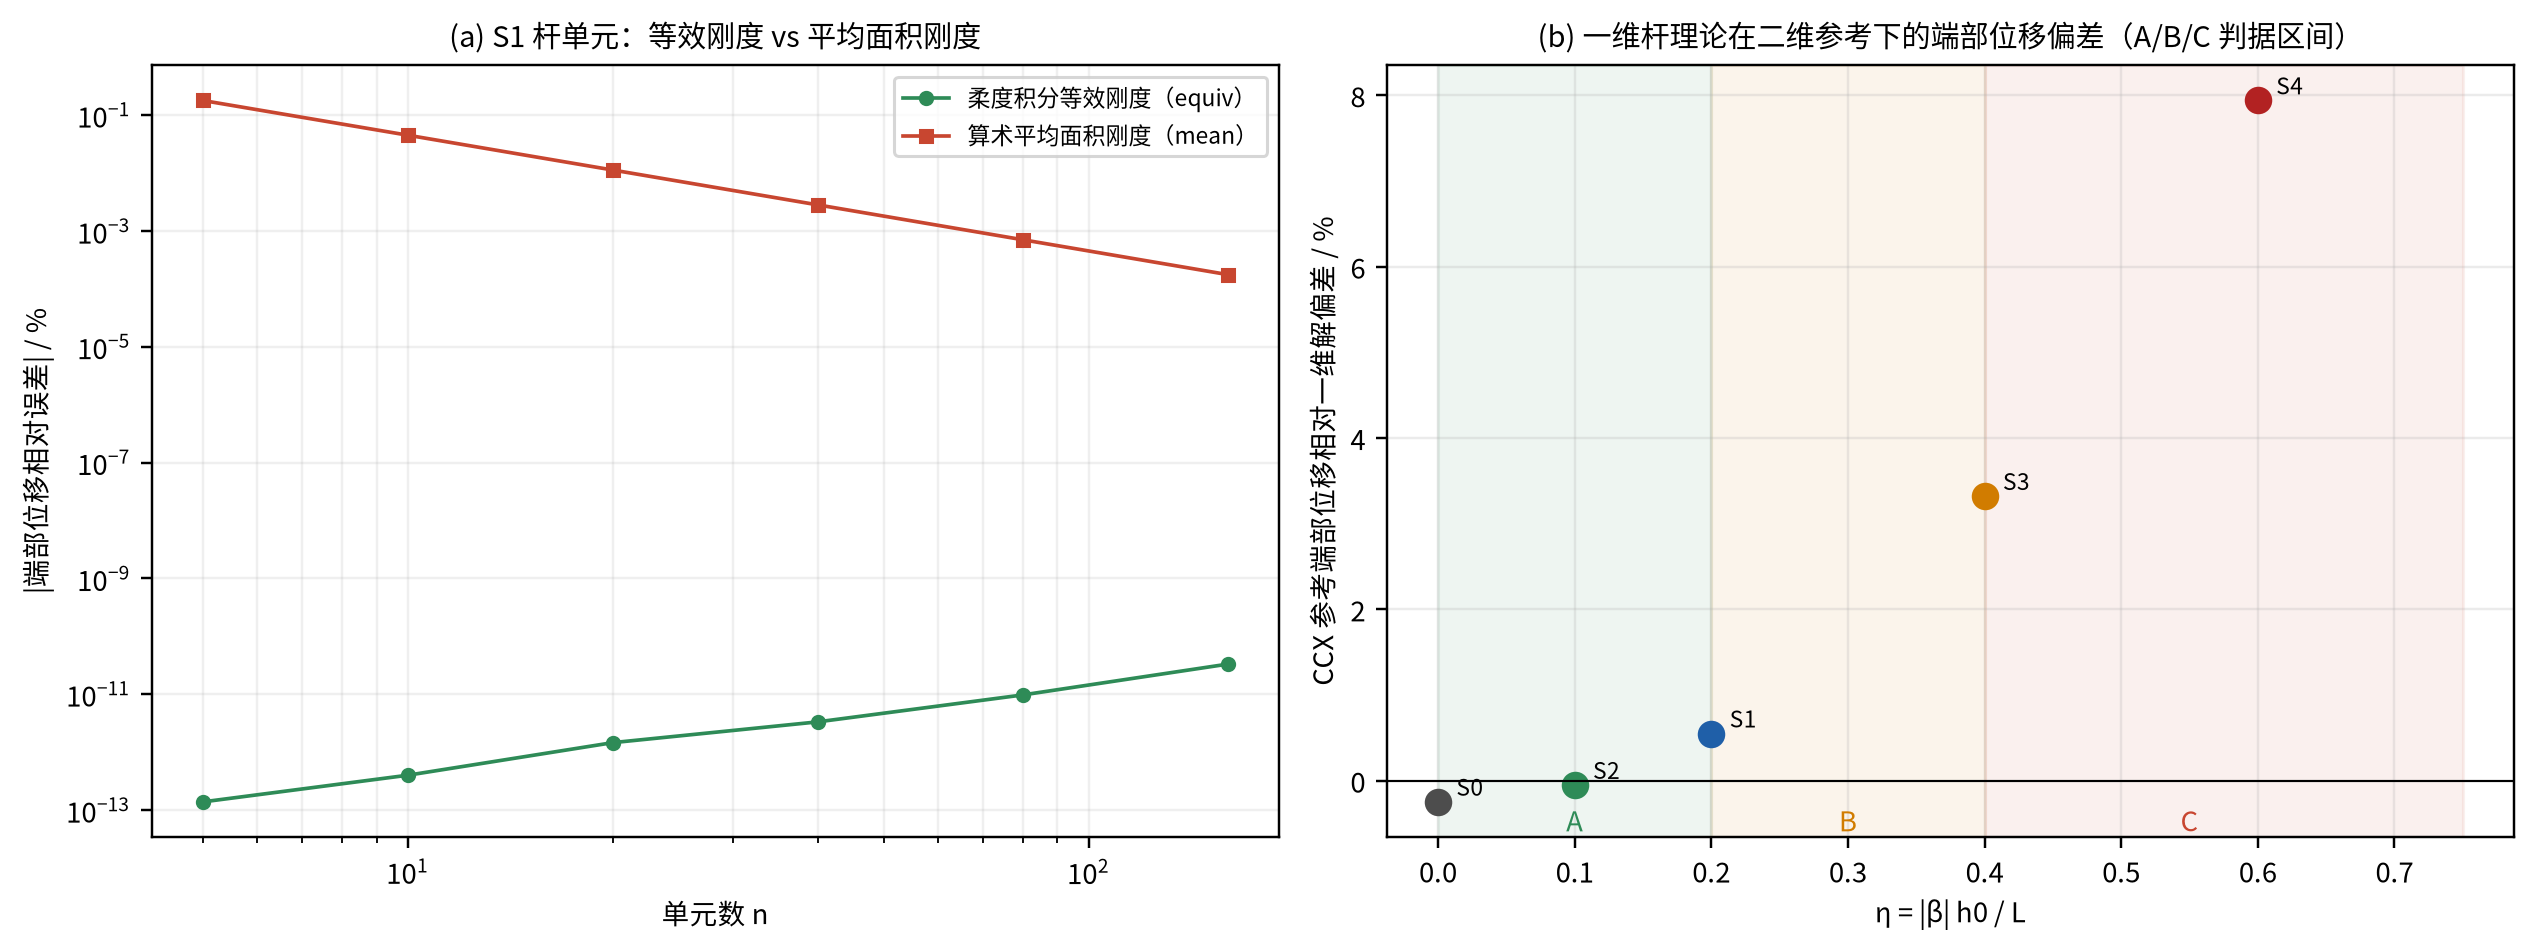
\includegraphics[width=\textwidth]{figures/fig07_bar.png}
  \caption{杆单元刚度对比与一维判据。现象：柔度积分等效刚度的端位移误差保持在 $10^{-11}\%$ 以下的舍入量级；平均面积刚度误差按 $O(h^2)$ 下降；二维参考下的一维端部偏差随 $\eta$ 从 $+0.25\%$ 变到 $-7.36\%$。解读：节点精确性只说明 1D 方程解对了，不能消除 1D 模型本身的模型误差；A/B/C 分级应结合 $\eta$ 与后验偏差，而不能只看网格收敛。}
  \label{fig:bar}
\end{figure}

\subsection{CalculiX 锚点与端载敏感性}
\label{sec:anchor}

CalculiX 的 CPS8 $240\times48$ 参考与自研 Q4/CST 高度一致：Q4 的端位移偏差为 $0.000$–$0.025\%$，CST 为 $0.001$–$0.075\%$（表~\ref{tab:anchor}、图~\ref{fig:anchor}）。同网格 CPS4 与 Q4 的端位移差最大 $0.049\%$，说明单元公式、组装、边界与载荷实现正确。端载从一致面力改为等分节点力时，$u_{\rm end}$ 变化不超过 $0.281\%$，但加载端局部节点应力可差 $1\%$–$8\%$（表~\ref{tab:load}），因此点值应力对比必须统一口径。

\begin{table}[htbp]
  \centering
  \caption{CalculiX CPS8 $240\times48$ 参考与自研方法的端位移对照（Q4/CST 取 $160\times32$）。}
  \label{tab:anchor}
  \small
  \begin{tabular}{@{}lS[table-format=1.4e-2]S[table-format=1.4e-2]S[table-format=+1.3]S[table-format=1.4e-2]S[table-format=+1.3]@{}}
\toprule
工况 & {CPS8 $u_{\rm end}$/m} & {Q4 $u_{\rm end}$/m} & {Q4 偏差/\%} & {CST $u_{\rm end}$/m} & {CST 偏差/\%} \\
\midrule
S0 & 2.4938e-07 & 2.4938e-07 & -0.000 & 2.4937e-07 & -0.005 \\
S1 & 1.7424e-07 & 1.7424e-07 & -0.000 & 1.7422e-07 & -0.011 \\
S2 & 3.4639e-07 & 3.4640e-07 & 0.002 & 3.4639e-07 & -0.001 \\
S3 & 8.9520e-08 & 8.9506e-08 & -0.016 & 8.9480e-08 & -0.045 \\
S4 & 9.8819e-08 & 9.8794e-08 & -0.025 & 9.8745e-08 & -0.075 \\
\bottomrule
\end{tabular}

\end{table}

\begin{table}[htbp]
  \centering
  \caption{端载离散口径敏感性：一致面力与等分节点力的绝对差（\%）。}
  \label{tab:load}
  \small
  \begin{tabular}{@{}lS[table-format=1.3]S[table-format=1.3]@{}}
\toprule
工况 & {$\Delta u_{\rm end}$/\%} & {$\Delta u_{\rm mid}$/\%} \\
\midrule
S0 & 0.016 & 0.000 \\
S1 & 0.062 & 0.000 \\
S2 & 0.001 & 0.000 \\
S3 & 0.207 & 0.015 \\
S4 & 0.281 & 0.017 \\
\bottomrule
\end{tabular}

\end{table}

\begin{figure}[htbp]
  \centering
  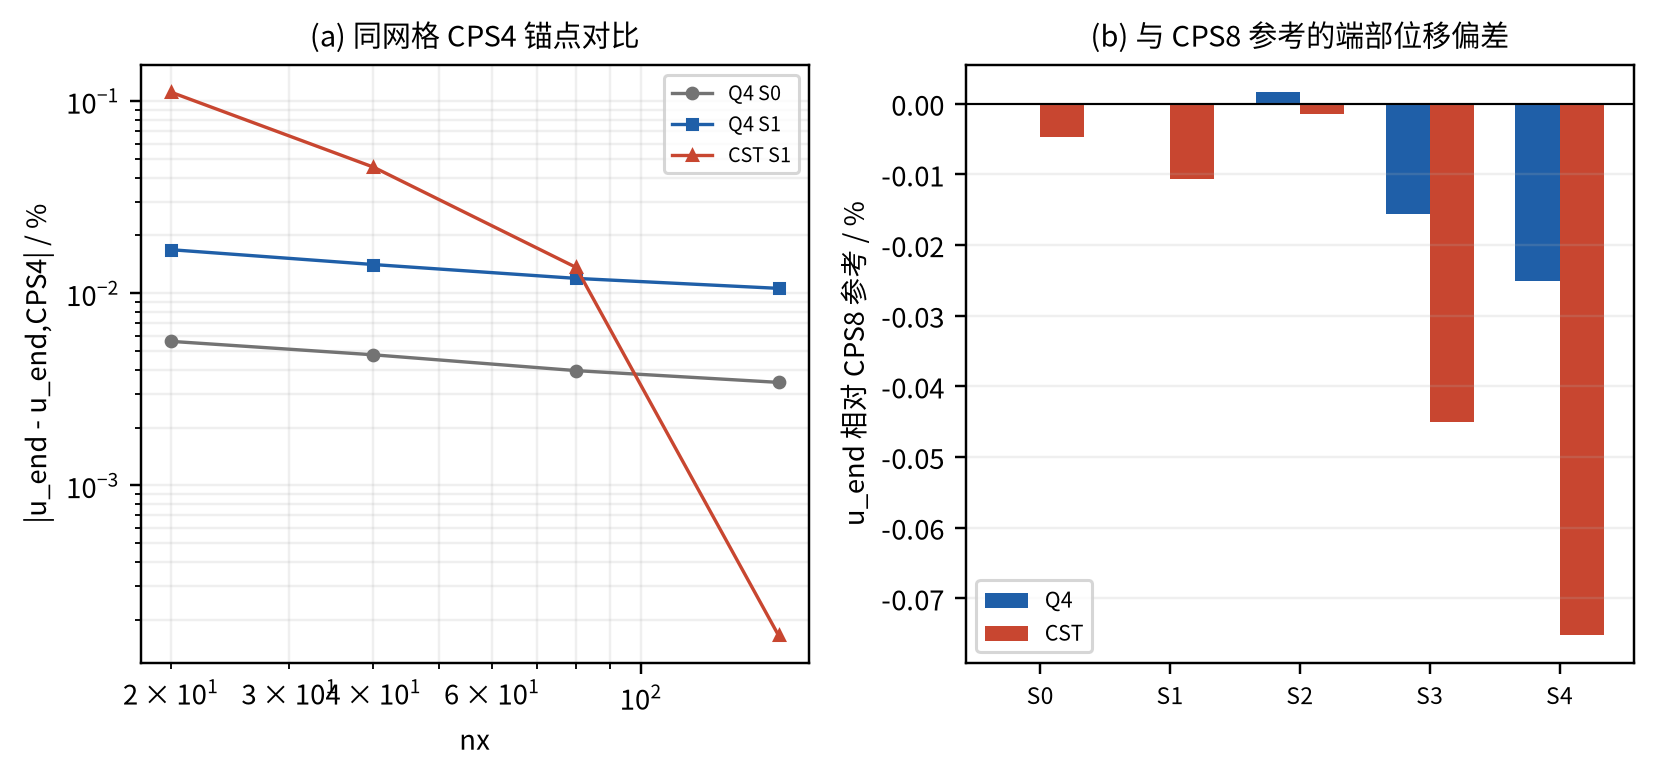
\includegraphics[width=\textwidth]{figures/fig08_anchor.png}
  \caption{与 CalculiX 的锚点对比。现象：同网格 Q4 与 CPS4 的差在 $10^{-2}\%$ 量级并随网格减小；CST 在粗网格的差明显更大，$160\times32$ 时降到 $10^{-3}\%$ 以下；自研 Q4/CST 与 CPS8 参考的端位移差均小于 $0.08\%$。解读：自研单元与 CalculiX 的实现一致，剩余差异来自 CalculiX 将平面应力单元展开为三维单元的厚度积分细节；CST 的粗网格差异主要来自常应变假设。}
  \label{fig:anchor}
\end{figure}

\subsection{FEniCS 可选本构校核}
\label{sec:fenics}

FEniCS/dolfinx 0.11 以 P2 三角形、$80\times16$ 网格、一致面力对 S0/S1 做独立校核：S0 的 $u_{\rm end}=2.493808\times10^{-7}\,\mathrm{m}$，与一维解的偏差来自固定端泊松约束；S1 的 $u_{\rm end}=1.742433\times10^{-7}\,\mathrm{m}$，与 CCX $240\times48$ 参考仅差 $+0.0029\%$。两个独立第三方求解器互证了锚点参考值（表~\ref{tab:fenics}）。

\begin{table}[htbp]
  \centering
  \caption{FEniCS 本构/位移校核（P2 三角形，$80\times16$）。}
  \label{tab:fenics}
  \small
  \begin{tabular}{@{}lS[table-format=1.4e-2]S[table-format=1.4e-2]S[table-format=+1.3]S[table-format=5.2]@{}}
\toprule
工况 & {FEniCS $u_{\rm end}$/m} & {1D $u_{\rm end}$/m} & {偏差/\%} & {$\sigma_{\rm mid}$/Pa} \\
\midrule
S0 & 2.4938e-07 & 2.5000e-07 & -0.248 & 50000.00 \\
S1 & 1.7424e-07 & 1.7329e-07 & 0.552 & 33445.12 \\
\bottomrule
\end{tabular}

\end{table}

\subsection{变形与应力云图}

S1 在 $40\times8$ 网格下的变形与 $\sigma_x$ 云图（图~\ref{fig:deformed}）显示：变形放大 $2.5\times10^5$ 后，楔形段整体伸长，$\sigma_x$ 从固定端到自由端逐渐降低，与 $P/A(x)$ 的趋势一致。

\begin{figure}[htbp]
  \centering
  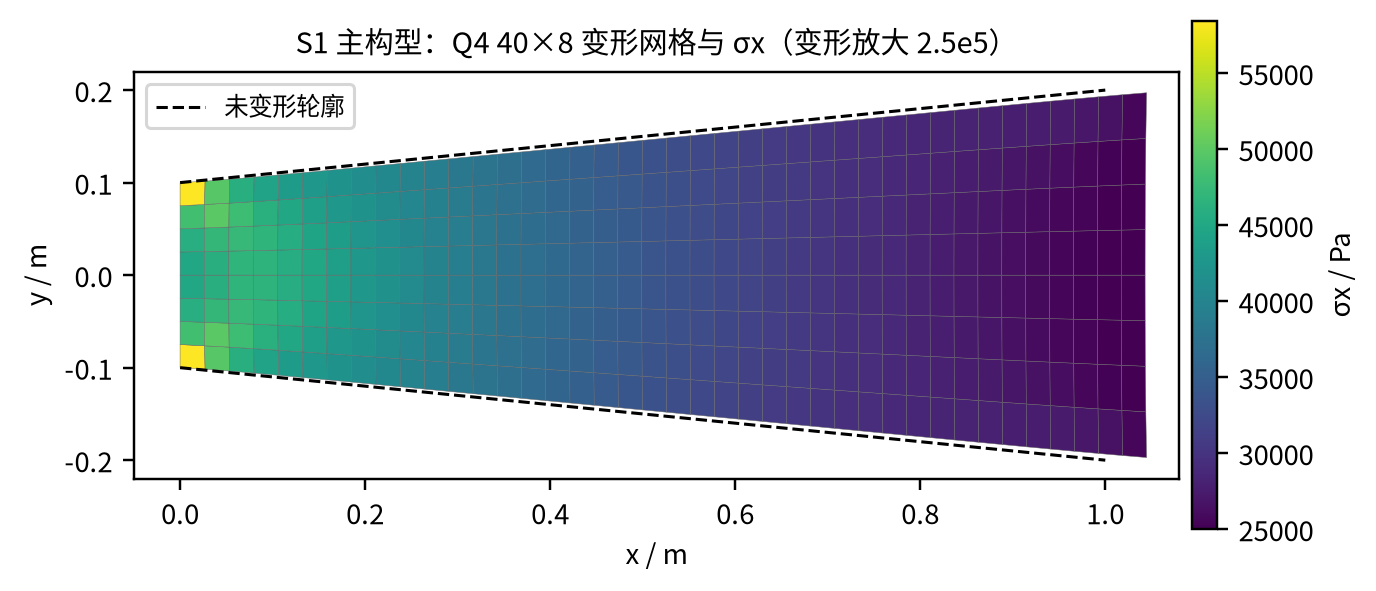
\includegraphics[width=0.86\textwidth]{figures/fig09_deformed.png}
  \caption{S1 的变形网格与 $\sigma_x$ 云图（Q4，$40\times8$，变形放大 $2.5\times10^5$）。现象：楔形段整体伸长，固定端附近出现明显的应力集中，自由端应力最低。解读：这正是二维模型相对一维杆的附加信息——一维杆只能给出截面平均值，无法显示端部与边缘的局部应力梯度。}
  \label{fig:deformed}
\end{figure}
\section{讨论}

\subsection{三种方法的精度与效率}

若以应力精度为主要目标，Q4 是三种方法中最均衡的选择。它在 $160\times32$ 网格上的探针应力误差不超过 $0.042\%$，明显低于 CST 的 $0.146\%$，且能直接给出单元内线性变化的应力场；代价是每节点两个自由度、单元数虽少但后处理更复杂。CST 的优势在实现简单与几何适应性，常应变假设使其偏刚，局部应力误差更大，且在粗网格上呈现明显的分块与对角线敏感性；若必须使用 CST，应配合面积加权节点恢复与更密网格。

杆单元的效率无可替代：每节点一个自由度，节点位移精确，且与网格无关。它的局限是只给出一维曲线，无法描述端部局部变形、横向应力与截面非均匀性；因此它适合 A/B 级工况的快速估算与趋势判断，不适合作为 C 级工况或端部强度评定的最终依据。工程上合理的流程是“一维杆快速估算 + Q4 二维复核 + 关键区域网格加密”，CST 则用于复杂几何的快速原型或与自动剖分工具对接。

\subsection{一维判据与边界层}

$\eta=|\beta|h_0/L=\tan\alpha$ 是一个纯几何判据，优点是可在建模前计算，缺点是没有包含端部约束与载荷分布的影响。本文用二维参考标定了 A/B/C 阈值，并给出对应的后验偏差；需要强调两点。第一，即使 $\eta=0$（等截面），固定端全约束仍造成约 $0.25\%$–$0.50\%$ 的位移偏差，这是圣维南边界层而非锥度效应，一维杆的截面平均应力仍精确等于 $P/A$。第二，A 级只承诺“内部/中截面可信、端部约 $1\%$”，不应把 A 级理解为“端部位移也准确”；若关心端部，必须做二维复核。

\subsection{口径敏感性}

本文量化了三类口径的影响，结论是：端载口径影响端部位移约 $0.02\%$–$0.28\%$，但影响加载端局部应力可达 $1\%$–$8\%$；截面平均口径（节点算术平均与面积加权）在粗网格上可差 $0.4\%$，并严重污染位移收敛阶；CST 后处理的 raw 与 recovered 差异主要出现在粗网格的截面内振荡。因此，跨方法/跨代码对比前必须统一端载、截面平均和应力恢复口径，否则很容易把后处理差异误判为方法误差。

\subsection{局限}

本文限定于线弹性、小变形、平面应力、对称楔形与端部均布载荷；未考虑三维效应、材料非线性、接触、动力与优化。CalculiX 平面应力单元通过三维展开实现，与严格二维平面应力在厚度积分细节上存在约 $0.01\%$–$0.05\%$ 的差异。CST 的对角线敏感性指标依赖镜像对称性；对非对称几何/载荷，全局量也会出现离散，需要按一般网格敏感性方法处理。此外，本文的“梯度保真误差”使用截面平均应力的中心差分，参考梯度来自 CPS8 细网格，其绝对值仍受参考解与差分算子影响，宜作为相对比较而非绝对误差。

\section{结论}

\begin{enumerate}[leftmargin=2em,itemsep=0.35em]
  \item 建立了变截面矩形拉杆的三种自写有限元方法，并用 CalculiX CPS4/CPS8 与 FEniCS 完成第三方锚点验证。同网格 Q4 与 CPS4 的端位移差不超过 $0.05\%$，FEniCS 对 S1 的端位移与 CCX 参考仅差 $+0.0029\%$，证明单元、组装、边界与载荷实现正确。
  \item 一维杆采用柔度积分等效刚度后，节点位移与解析解一致到 $10^{-13}$ 且与网格无关；平均面积刚度会高估刚度，粗网格端位移误差按 $O(h^2)$ 收敛。等截面退化校核（$\beta=0$）通过。
  \item Q4（$2\times2$ 全积分）在 $160\times32$ 下的位移偏差不超过 $0.025\%$、探针应力偏差不超过 $0.042\%$；位移收敛阶约 $1.7$–$2.5$，应力收敛阶约 $1.6$–$2.3$，梯度保真误差 $0.35\%$–$0.95\%$。
  \item CST 的全局量在对称工况下与剖分方向无关（离散度约 $10^{-11}\%$），局部单元应力对角离散度为 $0.2\%$–$1.1\%$；面积加权节点恢复在粗网格上显著降低截面内应力振荡，但不能替代网格加密。
  \item 一维判据 $\eta=|\beta|h_0/L$ 与二维参考一致：S0/S1/S2 为 A，S3 为 B，S4 为 C；一维杆端部偏差依次为 $+0.25\%$、$-0.55\%$、$+0.05\%$、$-3.21\%$、$-7.36\%$，中截面偏差为 $+0.50\%$、$-0.05\%$、$+0.29\%$、$-1.16\%$、$-4.10\%$。
  \item 推荐流程：A/B 级工况先用等效刚度杆单元估算轴力与位移，再用 Q4 复核端部；C 级工况必须使用二维模型；CST 适合快速原型/复杂几何，但需注意局部应力对剖分的敏感性。三种方法的产出形态差异（一维曲线、连续云图、分块云图）应作为选型的首要判据之一。
\end{enumerate}


\appendix
\section{复现命令与文件清单}

\subsection*{A.1 复现命令}

在项目根目录 \texttt{tapered\_bar} 下依次执行：
\begin{verbatim}
python3 tests/test_core.py
python3 tests/test_bar.py
python3 tests/test_q4.py
python3 tests/test_cst.py
python3 tests/test_ccx.py
python3 scripts/run_bar.py
python3 scripts/run_q4.py
python3 scripts/run_cst.py
python3 scripts/run_ccx.py
python3 scripts/run_study.py
python3 scripts/make_figures.py
python3 scripts/make_latex_figures.py
python3 scripts/make_latex_tables.py
\end{verbatim}
LaTeX 报告在 \texttt{latex/} 下用 XeLaTeX 编译：
\begin{verbatim}
cd latex && xelatex main.tex && xelatex main.tex
\end{verbatim}

\subsection*{A.2 文件清单}

\begin{itemize}[leftmargin=1.6em,itemsep=0.15em]
  \item \texttt{fem/}：共享核心与三种方法（\texttt{config, analytic, mesh, assembly, post, bar, q4, cst}）。
  \item \texttt{scripts/}：各方法驱动、统一研究、图表与 LaTeX 表格生成。
  \item \texttt{anchors/calculix/}：CalculiX 输入生成、运行与解析；\texttt{anchors/fenics/}：FEniCS 可选校核。
  \item \texttt{results/study\_*.csv}：统一口径的位移、应力、探针、收敛结果；\texttt{results/ccx\_*}：锚点与参考解。
  \item \texttt{figures/}：报告图；\texttt{latex/figures/}：LaTeX 使用的副本与新产出形态图。
  \item \texttt{latex/main.tex}、\texttt{latex/sections/*.tex}、\texttt{latex/tables/*.tex}：本报告源文件。
\end{itemize}


\begin{thebibliography}{9}
\bibitem{zienkiewicz2005}
O.~C. Zienkiewicz, R.~L. Taylor, J.~Z. Zhu.
\textit{The Finite Element Method: Its Basis and Fundamentals}. 6th ed.
Elsevier, 2005.

\bibitem{bathe2006}
K.-J. Bathe.
\textit{Finite Element Procedures}. Prentice Hall, 1996 (reprinted 2006).

\bibitem{hughes2000}
T.~J.~R. Hughes.
\textit{The Finite Element Method: Linear Static and Dynamic Finite Element Analysis}.
Dover, 2000.

\bibitem{dhondt2023}
G.~Dhondt.
\textit{CalculiX CrunchiX User's Manual}, Version 2.23, 2023.

\bibitem{alnaes2015}
M.~S. Aln{\ae}s, J.~Blechta, J.~Hake, et al.
The FEniCS Project Version 1.5.
\textit{Archive of Numerical Software}, 3(100), 2015.

\bibitem{fenicsx}
FEniCSx / DOLFINx documentation, version 0.11, 2026.
\end{thebibliography}


\end{document}